\section{Khám phá Dữ liệu (EDA) và Tiền xử lý Dữ liệu}

Dựa trên tệp đặc trưng \texttt{train\_features.csv} đã giới thiệu ở Chương 1, chương này tập trung phân tích khám phá dữ liệu (EDA) ban đầu, xây dựng quy trình tiền xử lý chuẩn hóa và kiểm toán dữ liệu sau xử lý. Toàn bộ quy trình được xây dựng nhất quán và thực thi thông qua notebook thực nghiệm \texttt{preprocessingforALL}. Nhằm mục đích đánh giá thực nghiệm xem việc tích hợp thêm ngữ cảnh khu vực địa lý có thực sự mang lại sự khác biệt và giúp cải thiện khả năng nhận diện bất thường hay không, nhóm nghiên cứu thiết lập quy trình tạo ra song song hai bộ dữ liệu thực nghiệm: bộ dữ liệu cơ sở (Baseline) và bộ dữ liệu mở rộng tương tác khu vực (Zone-enhanced).

\subsection{Khám phá Dữ liệu Ban đầu}

\subsubsection{Phân tích sự Mất cân bằng Lớp Dữ liệu}
Dữ liệu nhãn bất thường phản ánh trạng thái hoạt động của hệ thống phụ tải điện: $y=0$ tương ứng với trạng thái bình thường (\textit{Normal}) và $y=1$ tương ứng với trạng thái bất thường (\textit{Anomaly}). Thống kê trên toàn bộ $1.749.494$ bản ghi của tập dữ liệu \texttt{train\_features.csv} cho kết quả phân bố như sau:
\begin{itemize}
    \item \textbf{Lớp bình thường ($y=0$):} $1.712.198$ bản ghi, chiếm tỷ lệ xấp xỉ $97{,}87\%$.
    \item \textbf{Lớp bất thường ($y=1$):} $37.296$ bản ghi, chỉ chiếm tỷ lệ khoảng $2{,}13\%$.
\end{itemize}

\begin{figure}[H]
    \centering
    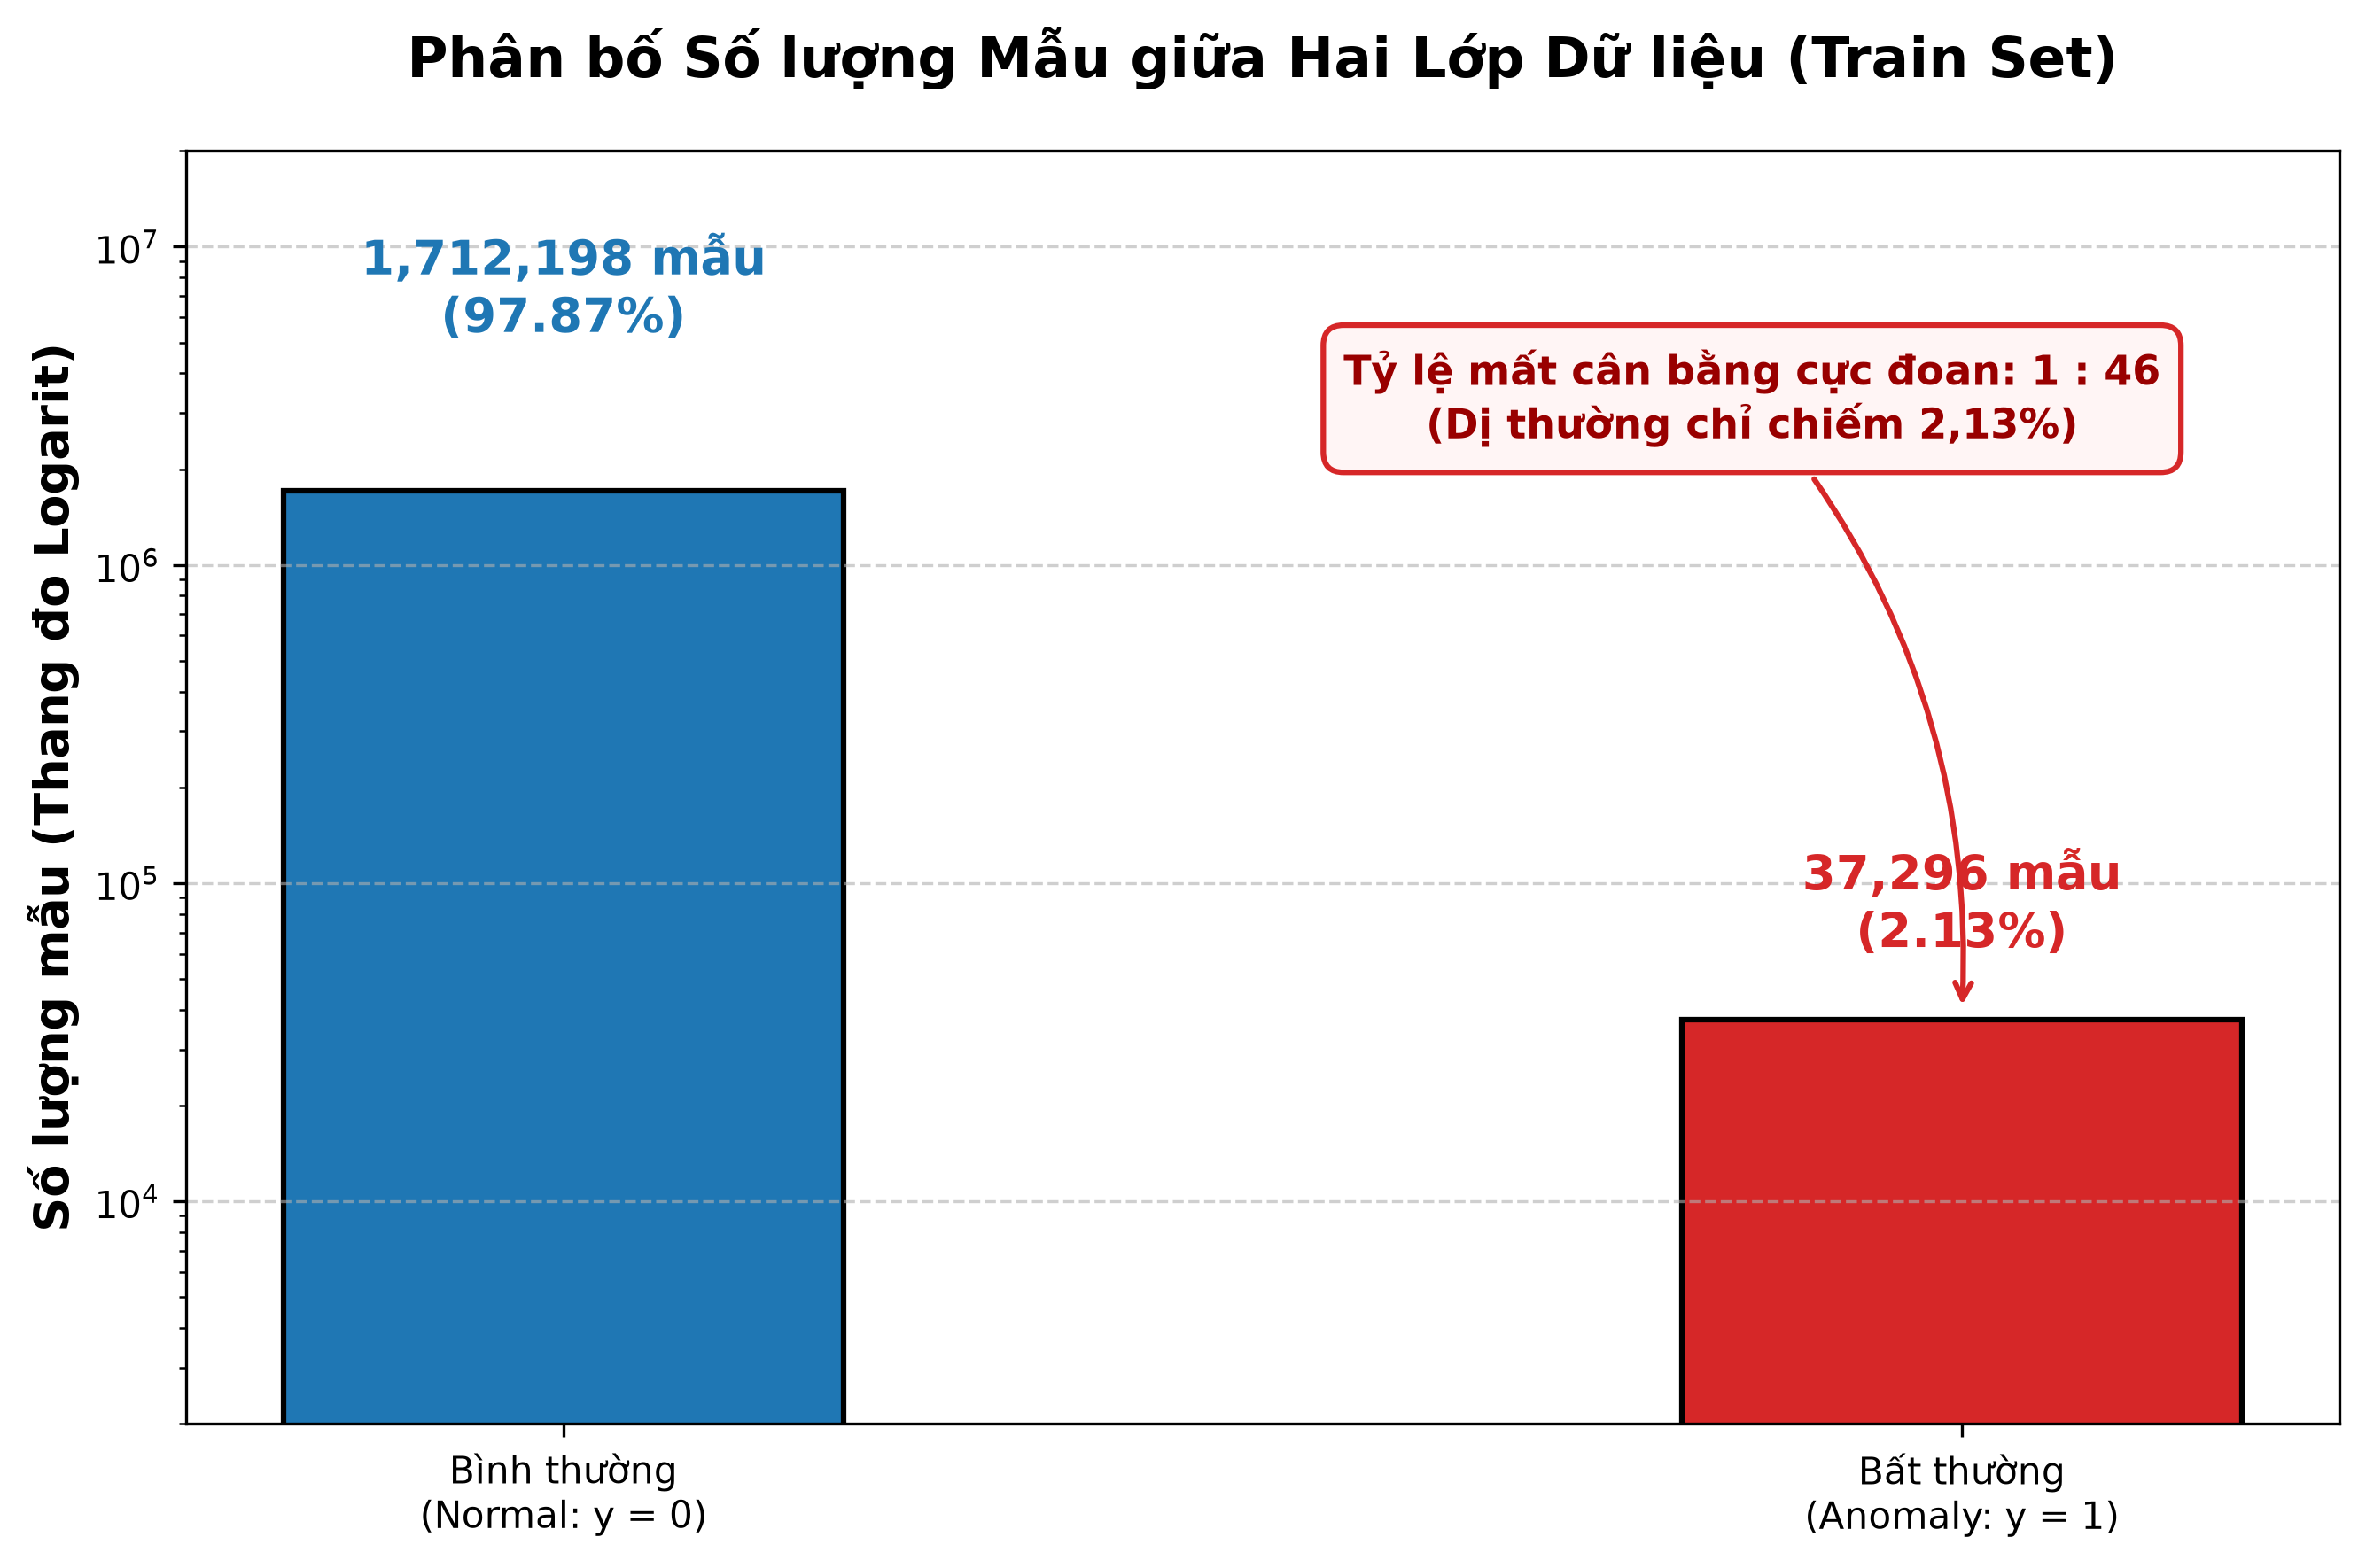
\includegraphics[width=0.68\textwidth]{IMAGE/eda_label_imbalance.png}
    \caption{\textbf{Phân phối mức độ mất cân bằng giữa nhãn bình thường và bất thường}}
    \label{fig:label_imbalance}
\end{figure}

Hình~\ref{fig:label_imbalance} trực quan hóa tỷ lệ mất cân bằng nghiêm trọng này thông qua biểu đồ cột trên thang đo logarit. Mức độ mất cân bằng tỷ lệ $1 : 46$ đặt ra thách thức kỹ thuật lớn:
\begin{enumerate}
    \item Nếu sử dụng hàm mất mát thông thường mà không điều chỉnh, mô hình sẽ có xu hướng tối ưu hóa bằng cách dự đoán toàn bộ mẫu là lớp đa số, dẫn đến chỉ số Accuracy rất cao nhưng hoàn toàn mất khả năng nhận diện các sự cố thực tế.
    \item Nếu sử dụng ngưỡng quyết định mặc định $\tau = 0{,}5$, đại đa số các mẫu dị thường có xác suất dự đoán trong khoảng $0{,}1 - 0{,}4$ sẽ bị bỏ sót, khiến chỉ số Recall và F1-Score bị suy giảm nghiêm trọng. Do đó, việc áp dụng kỹ thuật tối ưu hóa ngưỡng cắt xác suất (Threshold Moving) là điều kiện tiên quyết trong các giai đoạn sau.
\end{enumerate}

\subsubsection{Phân tích Phân phối Tần suất Đặc trưng qua Histogram Diagrams}

Bên cạnh sự mất cân bằng về số lượng bản ghi giữa các nhãn, việc thấu hiểu hình thái phân phối xác suất và mật độ tần suất của các thuộc tính định lượng gốc là yêu cầu mang tính quyết định trong giai đoạn Khám phá Dữ liệu (EDA). Nhóm nghiên cứu đã triển khai hàm phân tích \texttt{plot\_eda\_histogram\_distribution()} tại Bước 1 của quy trình để khởi tạo hệ thống lược đồ phân phối tần suất chuyên sâu (Hình~\ref{fig:eda_histogram_distribution}).

\begin{figure}[H]
    \centering
    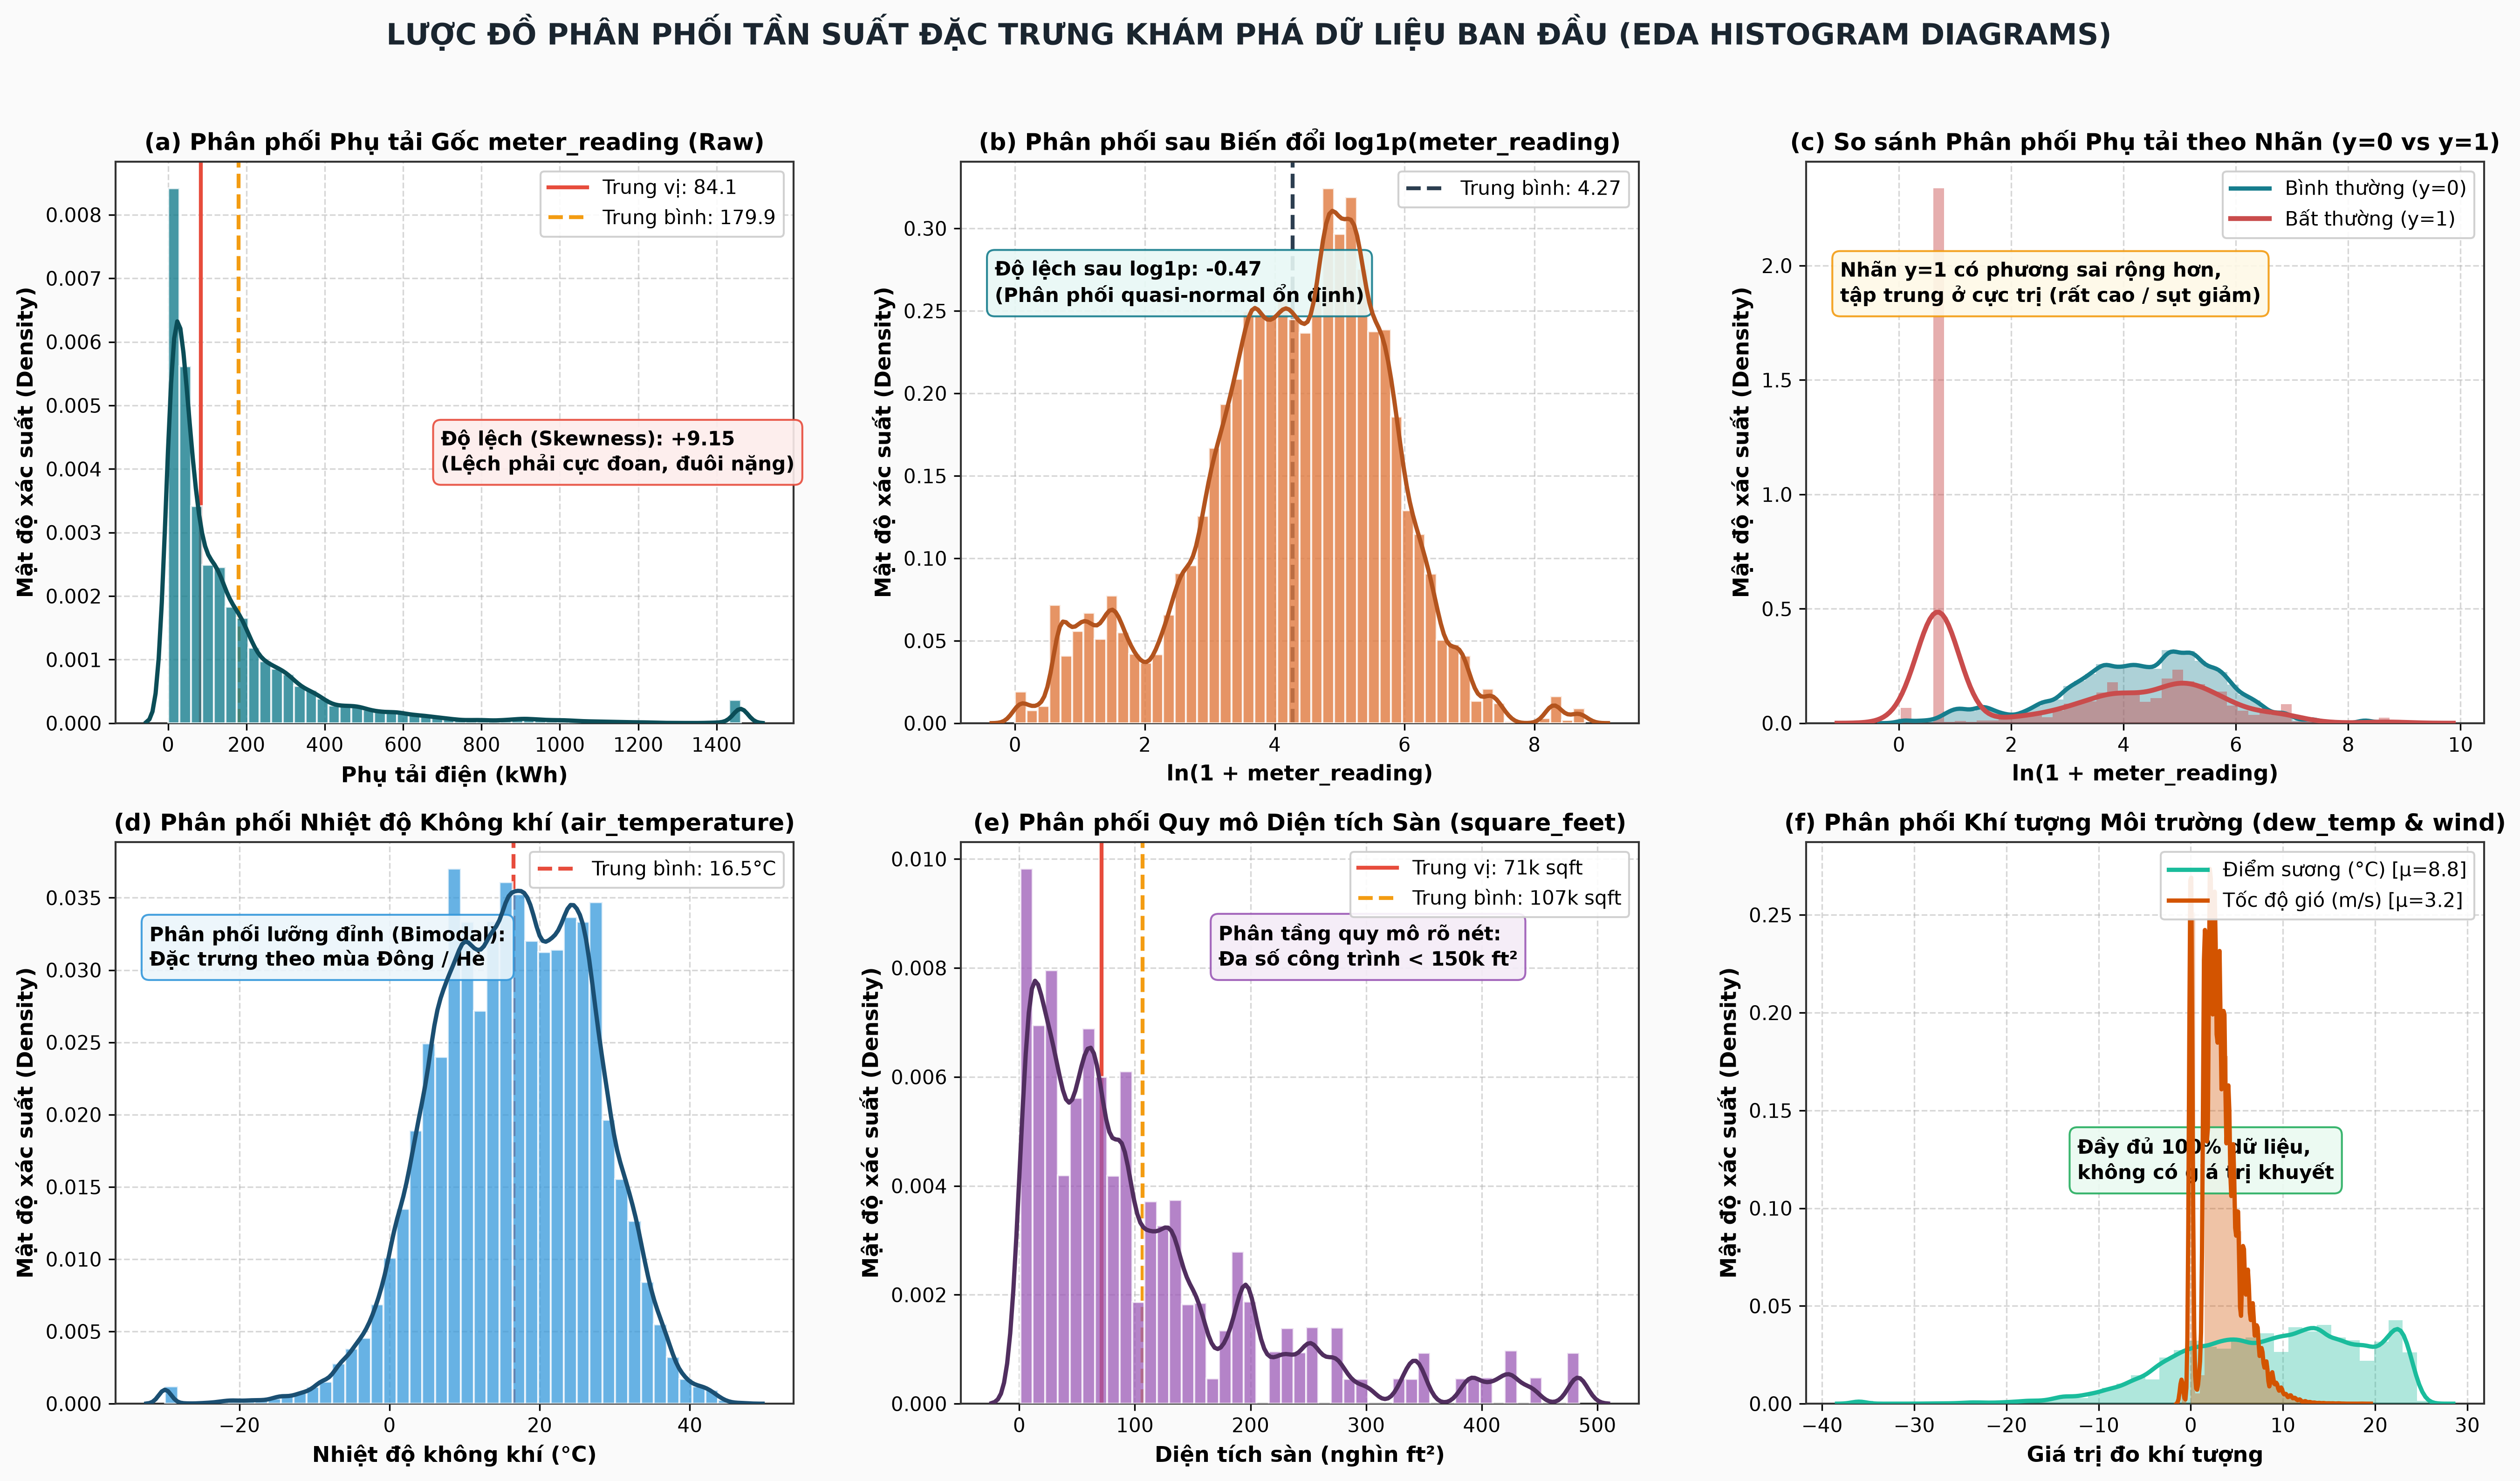
\includegraphics[width=0.98\textwidth]{IMAGE/eda_histogram_distribution.png}
    \caption{\textbf{Lược đồ Phân phối Tần suất Đặc trưng Khám phá Dữ liệu Ban đầu (EDA Histogram Diagrams)}}
    \label{fig:eda_histogram_distribution}
\end{figure}

Từ kết quả trực quan hóa tại Hình~\ref{fig:eda_histogram_distribution}, sáu đặc tính phân phối thống kê quan trọng được làm sáng tỏ:

\begin{enumerate}
    \item \textbf{Phân phối phụ tải gốc mang tính lệch phải cực đoan (Hình~\ref{fig:eda_histogram_distribution}a):}
    Thuộc tính tiêu thụ điện \texttt{meter\_reading} có độ lệch dương rất lớn ($\text{Skewness} = +9{,}15$) cùng phần đuôi phân phối dài và nặng. Phần lớn quan trắc tập trung ở dải phụ tải thấp với giá trị trung vị chỉ đạt $84{,}10\,\text{kWh}$, trong khi giá trị trung bình bị kéo lệch lên mức $179{,}90\,\text{kWh}$ do ảnh hưởng của các đỉnh tiêu thụ đột biến đạt tới $6.596{,}89\,\text{kWh}$. Đặc tính phân phối phi chuẩn này cho thấy các giải thuật giả định phân phối chuẩn như Naive Bayes hay Hồi quy tuyến tính sẽ kém hiệu quả và dễ bị thiên lệch nếu không qua bước biến đổi dữ liệu.

    \item \textbf{Tác động phục hồi tính chuẩn tắc của biến đổi Logarithm (Hình~\ref{fig:eda_histogram_distribution}b):}
    Khi áp dụng hàm nén phi tuyến $f(x) = \ln(1 + x)$, đuôi dài bên phải của phân phối được co cụm đáng kể, đưa độ lệch từ $+9{,}15$ về mức xấp xỉ đối xứng $-0{,}47$. Phân phối chuyển hóa thành hình chuông tựa chuẩn với kỳ vọng trung bình đạt $4{,}27$. Điều này cung cấp căn cứ toán học vững chắc cho việc sử dụng các mô hình cây quyết định phân nhánh trên thang đo logarit hoặc chuẩn hóa Z-score nhằm ổn định độ dốc gradient.

    \item \textbf{Sự phân hóa phân phối phụ tải theo trạng thái nhãn (Hình~\ref{fig:eda_histogram_distribution}c):}
    Khi bóc tách phân phối theo điều kiện $P(X \mid y=0)$ và $P(X \mid y=1)$:
    \begin{itemize}
        \item Lớp bình thường ($y=0$, màu xanh) phân bố tập trung dày đặc xung quanh mức tiêu thụ cơ sở ($3{,}5 - 5{,}5$ trên thang log, tương ứng $30 - 250\,\text{kWh}$).
        \item Ngược lại, lớp dị thường ($y=1$, màu đỏ) thể hiện phương sai cực rộng và xu hướng phân bố phân cực: Cực trị 1 sụt giảm sâu về cận 0 (tương ứng sự cố mất nguồn hoặc đứt tín hiệu cảm biến) và Cực trị 2 tăng vọt ở dải phụ tải đỉnh $> 6{,}5$ (tương ứng sự cố quá tải, chập điện). Sự chồng lấn phân phối này minh chứng rằng không thể dùng bất kỳ ngưỡng cắt tĩnh đơn biến nào để phát hiện dị thường mà bắt buộc phải kết hợp chuỗi đặc trưng đa biến.
    \end{itemize}

    \item \textbf{Tính chất phân phối lưỡng đỉnh của nhiệt độ môi trường (Hình~\ref{fig:eda_histogram_distribution}d):}
    Biến thời tiết \texttt{air\_temperature} thể hiện rõ nét hình thái phân phối hai đỉnh với kỳ vọng trung bình $16{,}5^\circ\text{C}$. Đỉnh thứ nhất tập trung quanh vùng $8^\circ\text{C} - 12^\circ\text{C}$ (đại diện cho mùa đông và khung giờ ban đêm), trong khi đỉnh thứ hai tập trung quanh $24^\circ\text{C} - 28^\circ\text{C}$ (mùa hè và khung giờ ban ngày). Sự phân hóa lưỡng cực này giải thích vì sao nhu cầu điện làm mát và sưởi ấm biến động theo mùa, tạo động lực cho việc xây dựng các biến chu kỳ tuần hoàn ($\sin/\cos$) ở Bước 2 tiền xử lý.

    \item \textbf{Sự phân tầng quy mô công trình đô thị (Hình~\ref{fig:eda_histogram_distribution}e):}
    Phân phối diện tích sàn \texttt{square\_feet} thể hiện tính phân tầng rõ rệt: giá trị trung vị đạt $71.000\,\text{ft}^2$, trong khi trung bình là $107.000\,\text{ft}^2$. Đại đa số công trình tập trung ở quy mô vừa và nhỏ ($< 150.000\,\text{ft}^2$, chủ yếu là văn phòng và trường học), trong khi một tỷ lệ nhỏ các công trình công cộng và trung tâm dữ liệu có diện tích vượt mức $400.000\,\text{ft}^2$, tạo ra tải nền tiêu thụ liên tục suốt ngày đêm.

    \item \textbf{Tính toàn vẹn của các thuộc tính khí tượng bổ trợ (Hình~\ref{fig:eda_histogram_distribution}f):}
    Phân phối của điểm sương \texttt{dew\_temperature} (trung bình $8{,}8^\circ\text{C}$) và tốc độ gió \texttt{wind\_speed} (trung bình $3{,}2\,\text{m/s}$) đạt độ toàn vẹn $100\%$ ($0$ giá trị khuyết), cho thấy dữ liệu khí tượng có tính ổn định cao, là nguồn tham chiếu môi trường đáng tin cậy.
\end{enumerate}

\subsubsection{Toàn cảnh Lịch sử Phụ tải và Phân bố Dị thường theo Thời gian}
Nhằm nắm bắt toàn diện hành vi phụ tải ở cấp độ vĩ mô và sự phân bố của các biến cố dị thường xuyên suốt 366 ngày trong năm 2016, nhóm nghiên cứu xây dựng lược đồ lịch sử vận hành trên toàn bộ 200 tòa nhà thuộc tập huấn luyện (Hình~\ref{fig:eda_history_diagram}).

\begin{figure}[H]
    \centering
    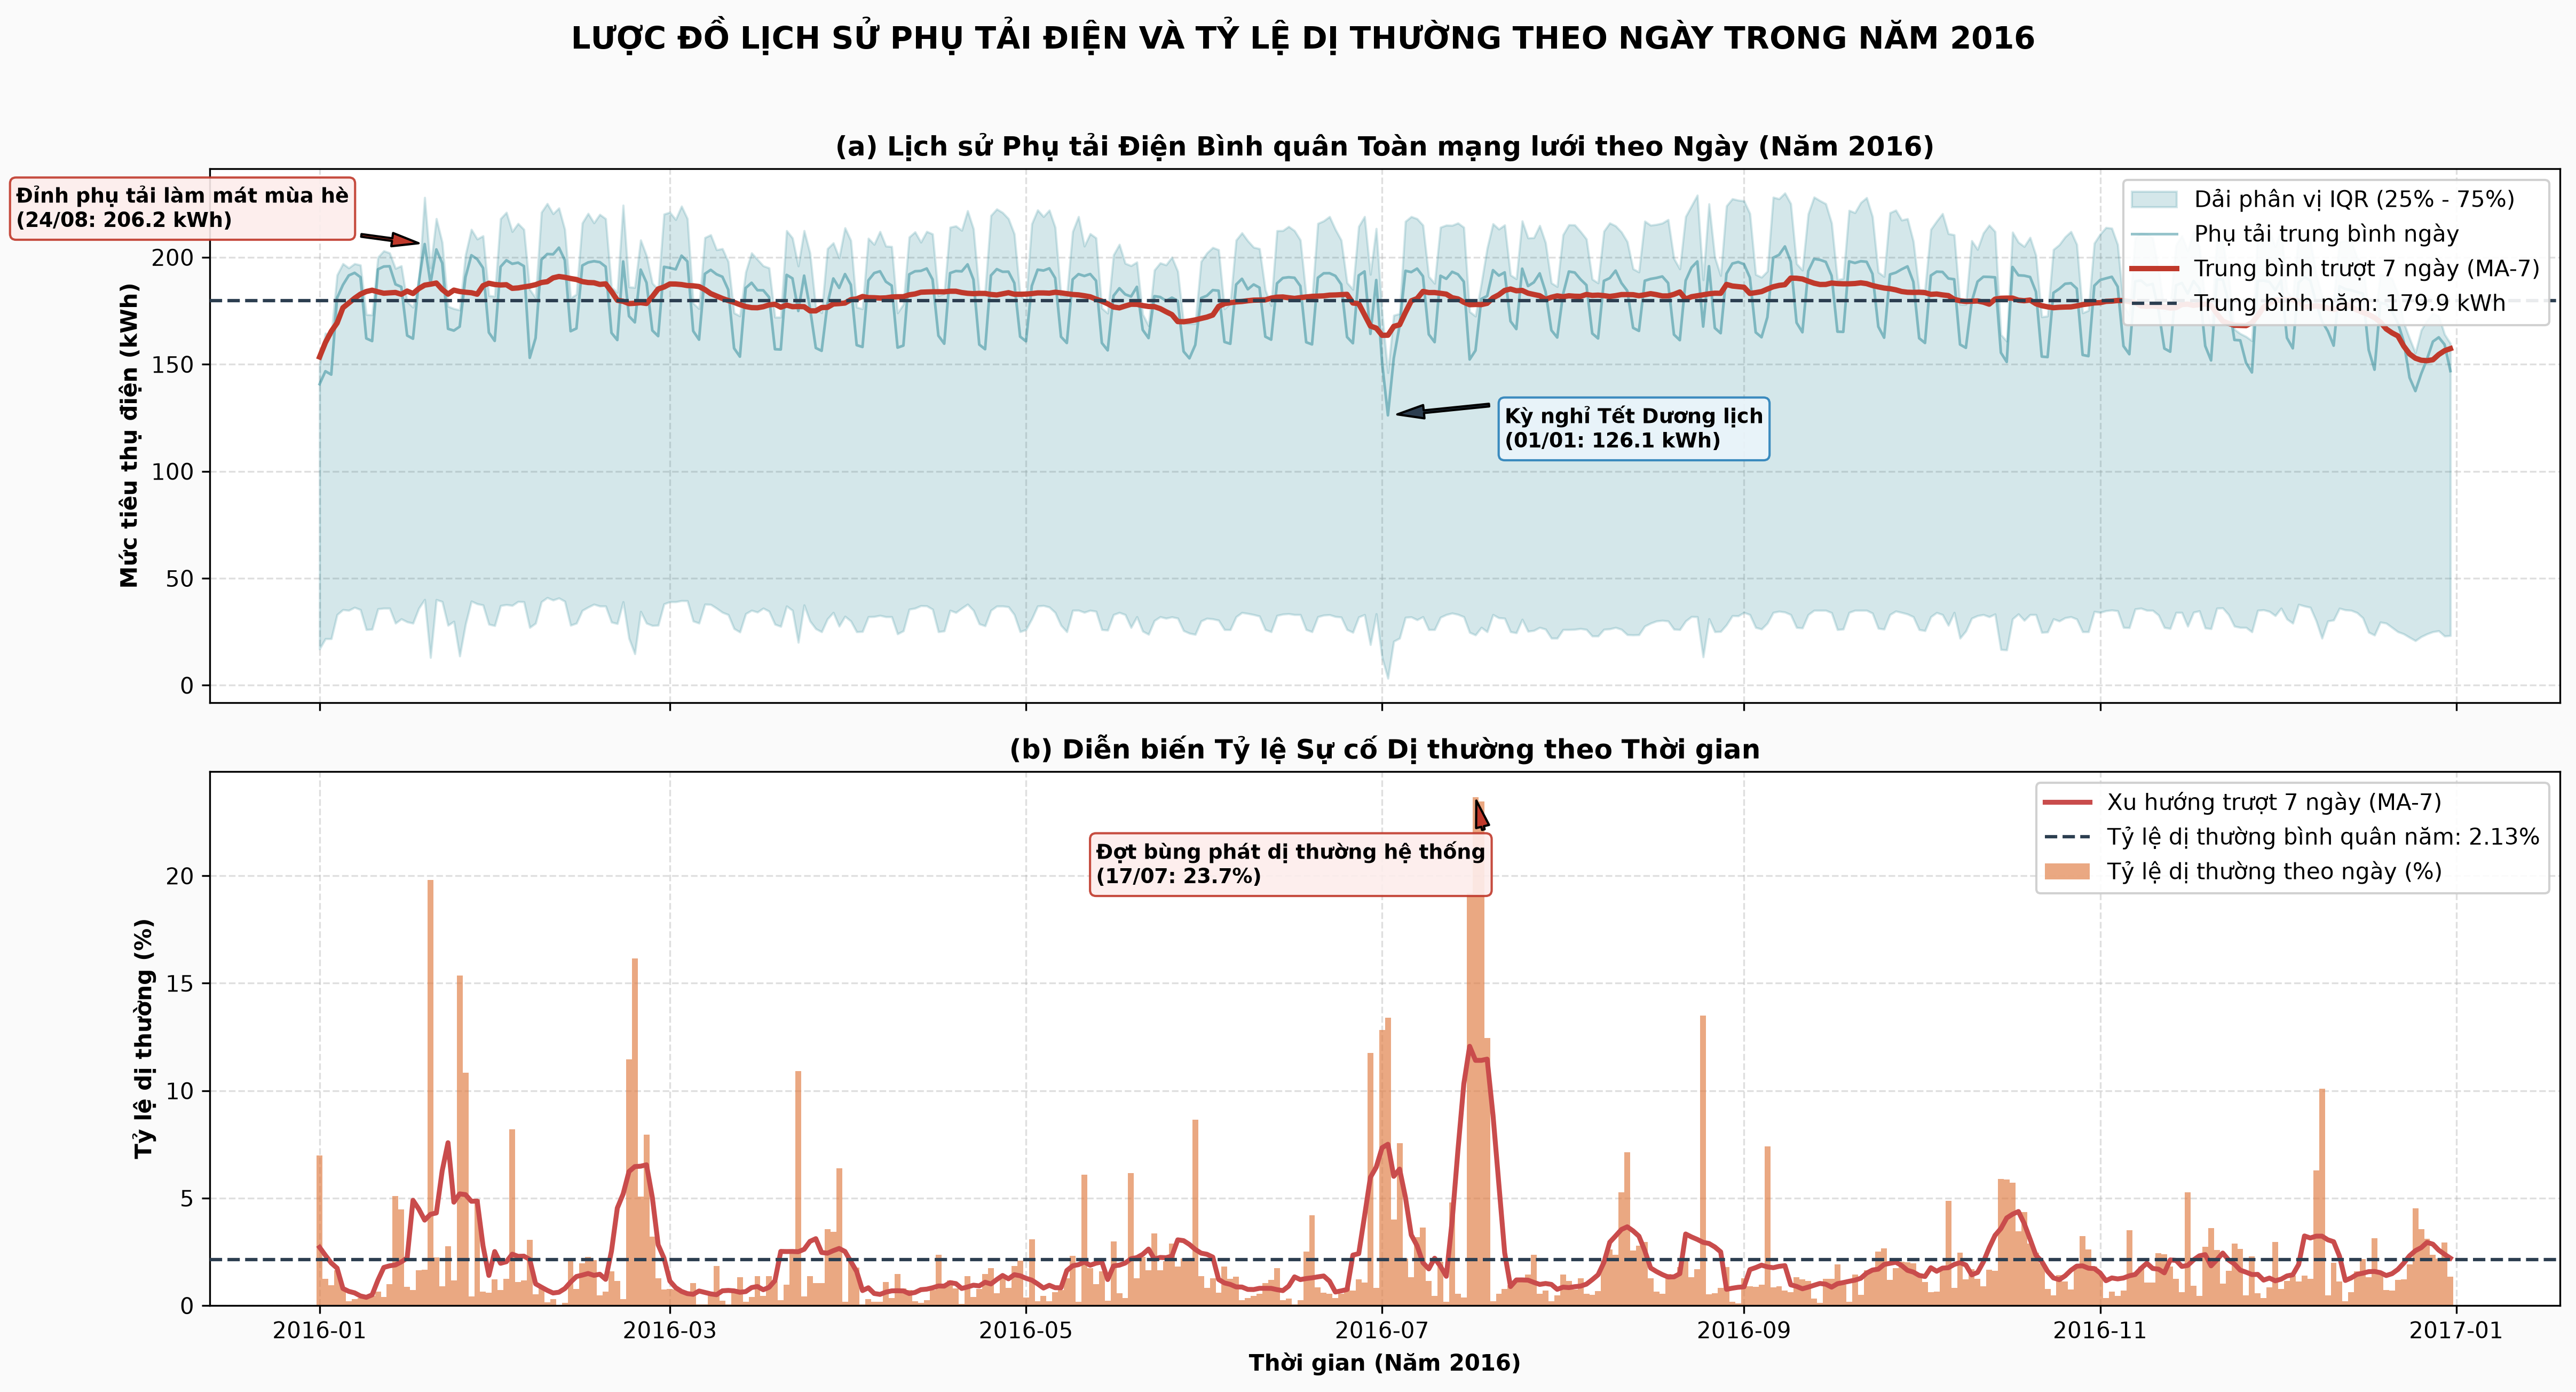
\includegraphics[width=0.98\textwidth]{IMAGE/eda_history_diagram.png}
    \caption{\textbf{Lược đồ Lịch sử Phụ tải Điện và Tỷ lệ Dị thường theo Ngày trong năm 2016}}
    \label{fig:eda_history_diagram}
\end{figure}

Từ lược đồ lịch sử vĩ mô tại Hình~\ref{fig:eda_history_diagram}, hai quy luật vận hành then chốt được khám phá:
\begin{enumerate}
    \item \textbf{Đặc thù lịch sử phụ tải trung bình ngày (biểu đồ trên):}
    \begin{itemize}
        \item Mức tiêu thụ điện bình quân toàn hệ thống đạt mức trung bình $179{,}88\,\text{kWh}$. Đường trung bình trượt 7 ngày (đường màu đỏ, tính bình quân theo từng tuần để triệt tiêu dao động giữa ngày làm việc và cuối tuần) cho thấy xu hướng phụ tải tăng cao rõ rệt vào các tháng mùa hè (tháng 6 đến tháng 8), đạt đỉnh $198{,}1\,\text{kWh}$ vào ngày 24/08/2016 do nhu cầu vận hành tối đa của hệ thống làm mát trung tâm (HVAC). Ngược lại, vào các kỳ nghỉ lễ lớn như Tết Dương lịch (01/01/2016) hoặc kỳ nghỉ mùa đông, mức tiêu thụ sụt giảm sâu xuống $140{,}7\,\text{kWh}$ do các hoạt động làm việc và học tập tạm ngưng.
        \item Dải phân vị IQR (nền xanh nhạt) phản ánh sự phân hóa mạnh mẽ về quy mô công trình: các tòa nhà giáo dục và văn phòng nhỏ duy trì phụ tải nền thấp ($20 - 40\,\text{kWh}$), trong khi các cơ sở phức hợp lớn tiêu thụ liên tục trên $200\,\text{kWh}$.
    \end{itemize}
    \item \textbf{Đặc thù lịch sử xuất hiện dị thường theo thời gian (biểu đồ dưới):}
    \begin{itemize}
        \item Mặc dù tỷ lệ dị thường bình quân cả năm chỉ là $2{,}14\%$ (đường chấm đen), các điểm dị thường không phân bố ngẫu nhiên đồng đều mà tập trung thành từng đợt sự cố hệ thống kéo dài nhiều ngày liên tiếp.
        \item Tiêu biểu nhất là đợt bùng phát dị thường vào trung tuần tháng 7 (đạt đỉnh $23{,}7\%$ vào ngày 17/07/2016) và các đợt biến động mạnh vào tháng 2, 3. Hiện tượng cụm dị thường theo thời gian chứng minh rằng việc mô hình hóa chuỗi thời gian thông qua các đặc trưng trễ, trung bình trượt, và tương tác vùng khí hậu là hoàn toàn cần thiết để phát hiện kịp thời các sự cố mang tính chuỗi.
    \end{itemize}
\end{enumerate}

\subsubsection{Phân loại Hình thái Dị thường Phụ tải trên Chuỗi Thời gian}
Trong khi Mục~3.1.3 quan sát xu hướng dài hạn theo ngày trên toàn mạng lưới, mục này đi sâu vào độ phân giải từng giờ tại công trình đại diện Tòa nhà \#439, Hình~\ref{fig:anomaly_timeseries} nhằm nhận diện quy luật phụ tải cơ sở và phân loại các hình thái dị thường thực tế.

\begin{figure}[H]
    \centering
    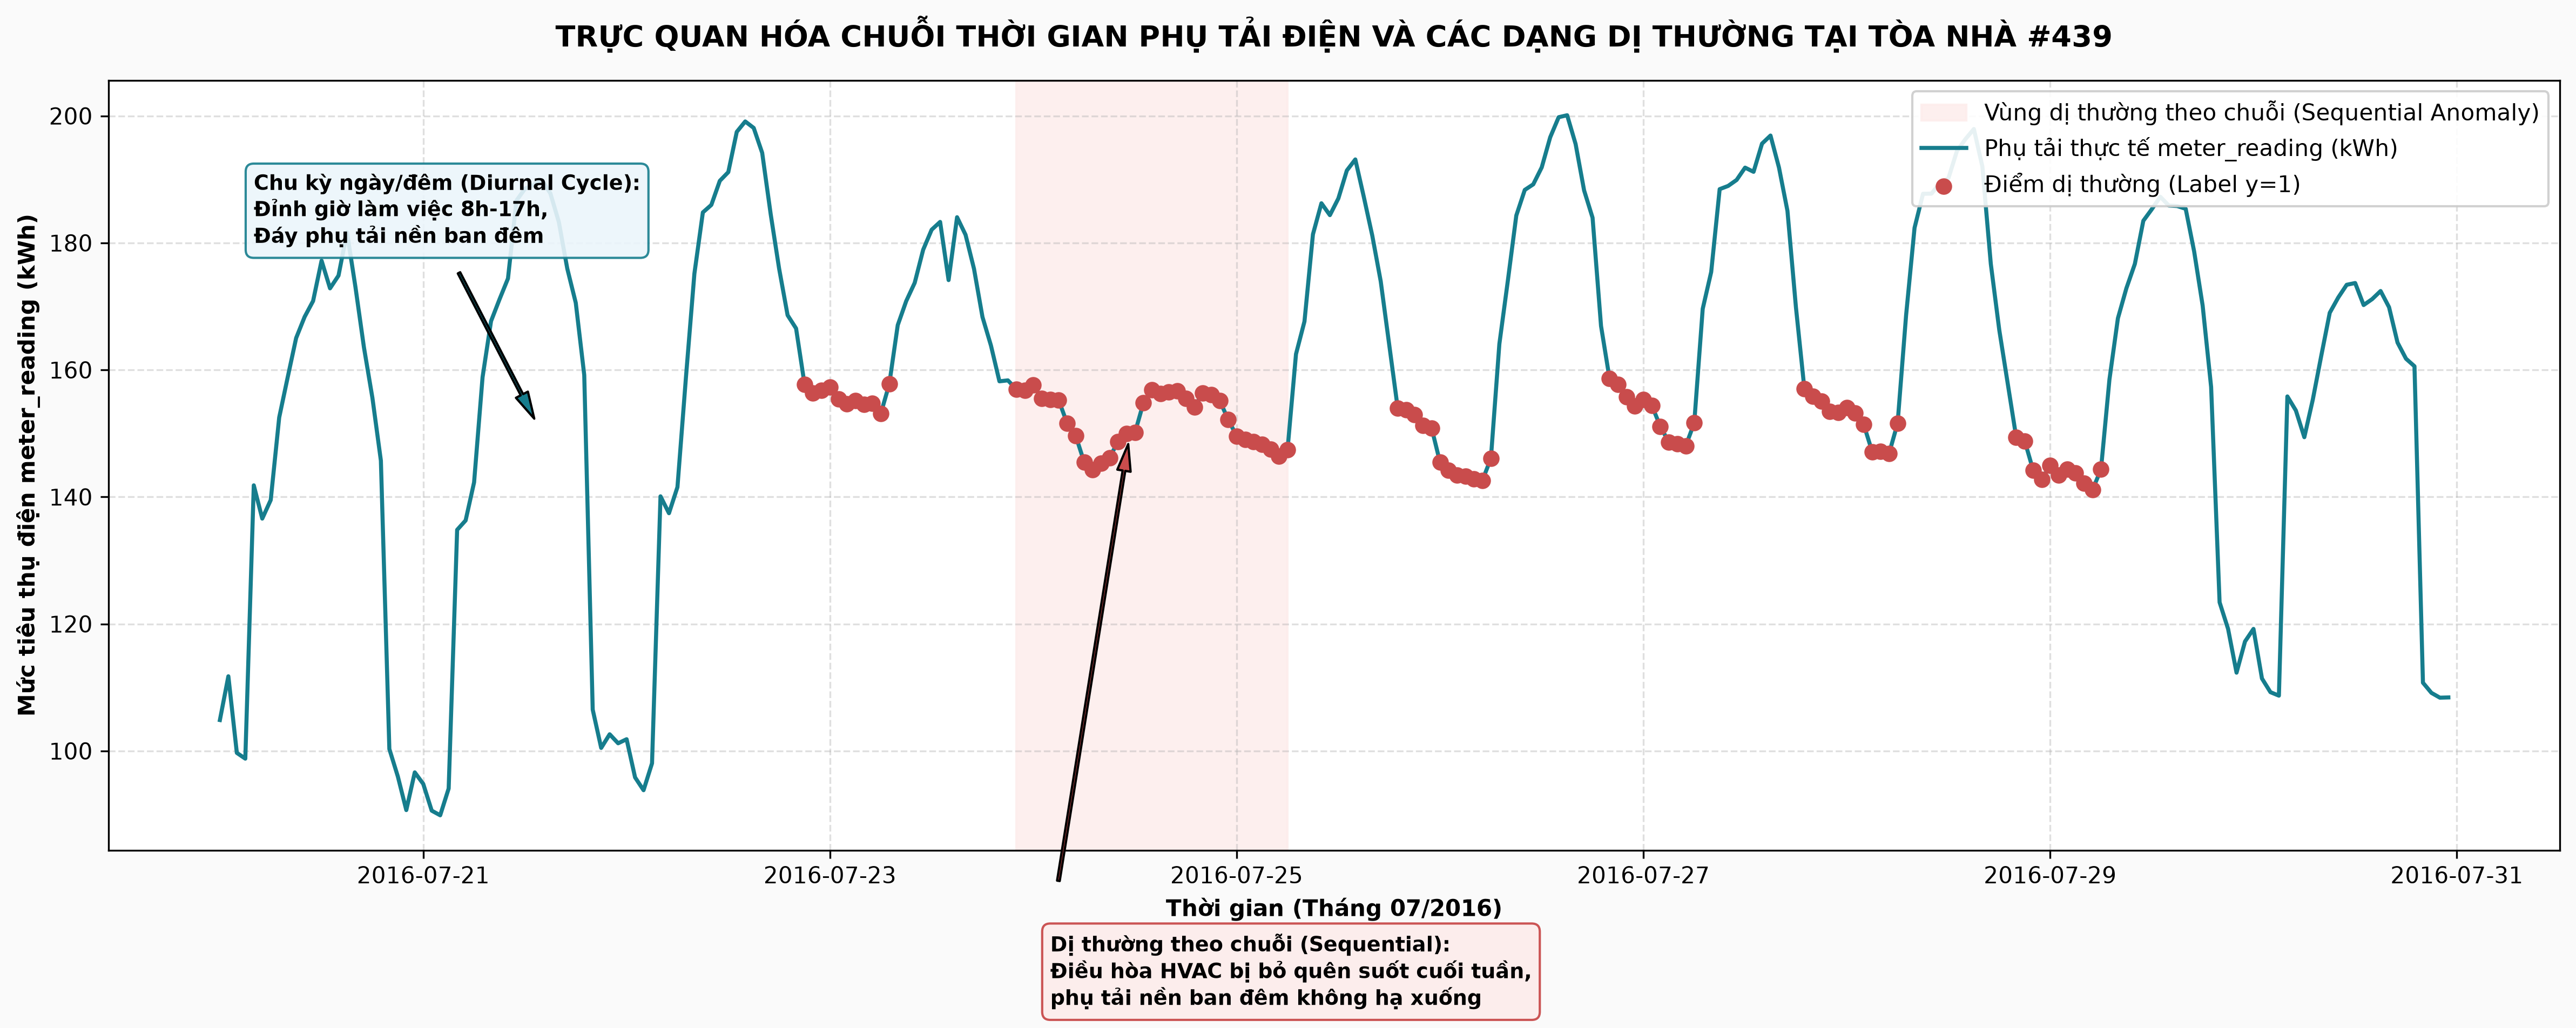
\includegraphics[width=0.98\textwidth]{IMAGE/eda_anomaly_timeseries.png}
    \caption{\textbf{Chuỗi thời gian phụ tải điện theo giờ và các dạng dị thường tại Tòa nhà \#439}}
    \label{fig:anomaly_timeseries}
\end{figure}

Chuỗi thời gian phụ tải theo giờ thể hiện hai chu kỳ sinh hoạt cơ sở: chu kỳ 24 giờ ngày/đêm, đỉnh phụ tải vào giờ làm việc 8h - 17h và đáy phụ tải nền vào ban đêm, cùng chu kỳ tuần, mức phụ tải giảm sút rõ rệt vào cuối tuần. Dựa trên sự sai lệch so với hai quy luật này, các điểm dị thường trong dữ liệu được phân chia thành hai nhóm:

\begin{enumerate}
    \item \textbf{Dị thường điểm (Point Anomaly):} Biểu hiện qua các xung đột biến tức thời tăng vọt hoặc sụt giảm về 0 đột ngột trong một vài giờ lẻ. Nguyên nhân thường xuất phát từ sự cố chập tải cục bộ, khởi động thiết bị công suất cực lớn không báo trước, hoặc cảm biến đo bị ngắt quãng tín hiệu tức thời.
    \item \textbf{Dị thường theo chuỗi (Sequential / Collective Anomaly):} Biểu hiện qua một đoạn liên tục nhiều giờ hoặc nhiều ngày mà mức tiêu thụ điện giữ nguyên ở mức cao bất thường (ví dụ: hệ thống điều hòa trung tâm bị bỏ quên không tắt trong suốt chuỗi ngày cuối tuần, thể hiện rõ tại Hình~\ref{fig:anomaly_timeseries}), hoặc phụ tải dao động hỗn loạn phá vỡ hoàn toàn chu kỳ ngày/đêm thông thường. Dạng dị thường này đòi hỏi mô hình phải kết hợp các đặc trưng trễ, biến chu kỳ lượng giác và độ lệch chuẩn trượt để nhận diện.
\end{enumerate}

\subsubsection{Nhiễu Cảm biến và Tình trạng Thiếu Dữ liệu}
Bên cạnh bài toán mất cân bằng nhãn, tình trạng nhiễu và đứt gãy tín hiệu đo lường từ đồng hồ thông minh là thách thức lớn thứ hai được phát hiện qua bước EDA. Nhóm nghiên cứu đã triển khai hàm \texttt{plot\_eda\_missing\_sensor\_noise()} tại Bước 1 để phân tích toàn diện hiện tượng này trên Tập Huấn luyện (\texttt{train\_features.csv}, $1.749.494$ bản ghi). Kết quả thống kê chi tiết được trực quan hóa tại Hình~\ref{fig:missing_sensor_noise}.

\begin{figure}[H]
    \centering
    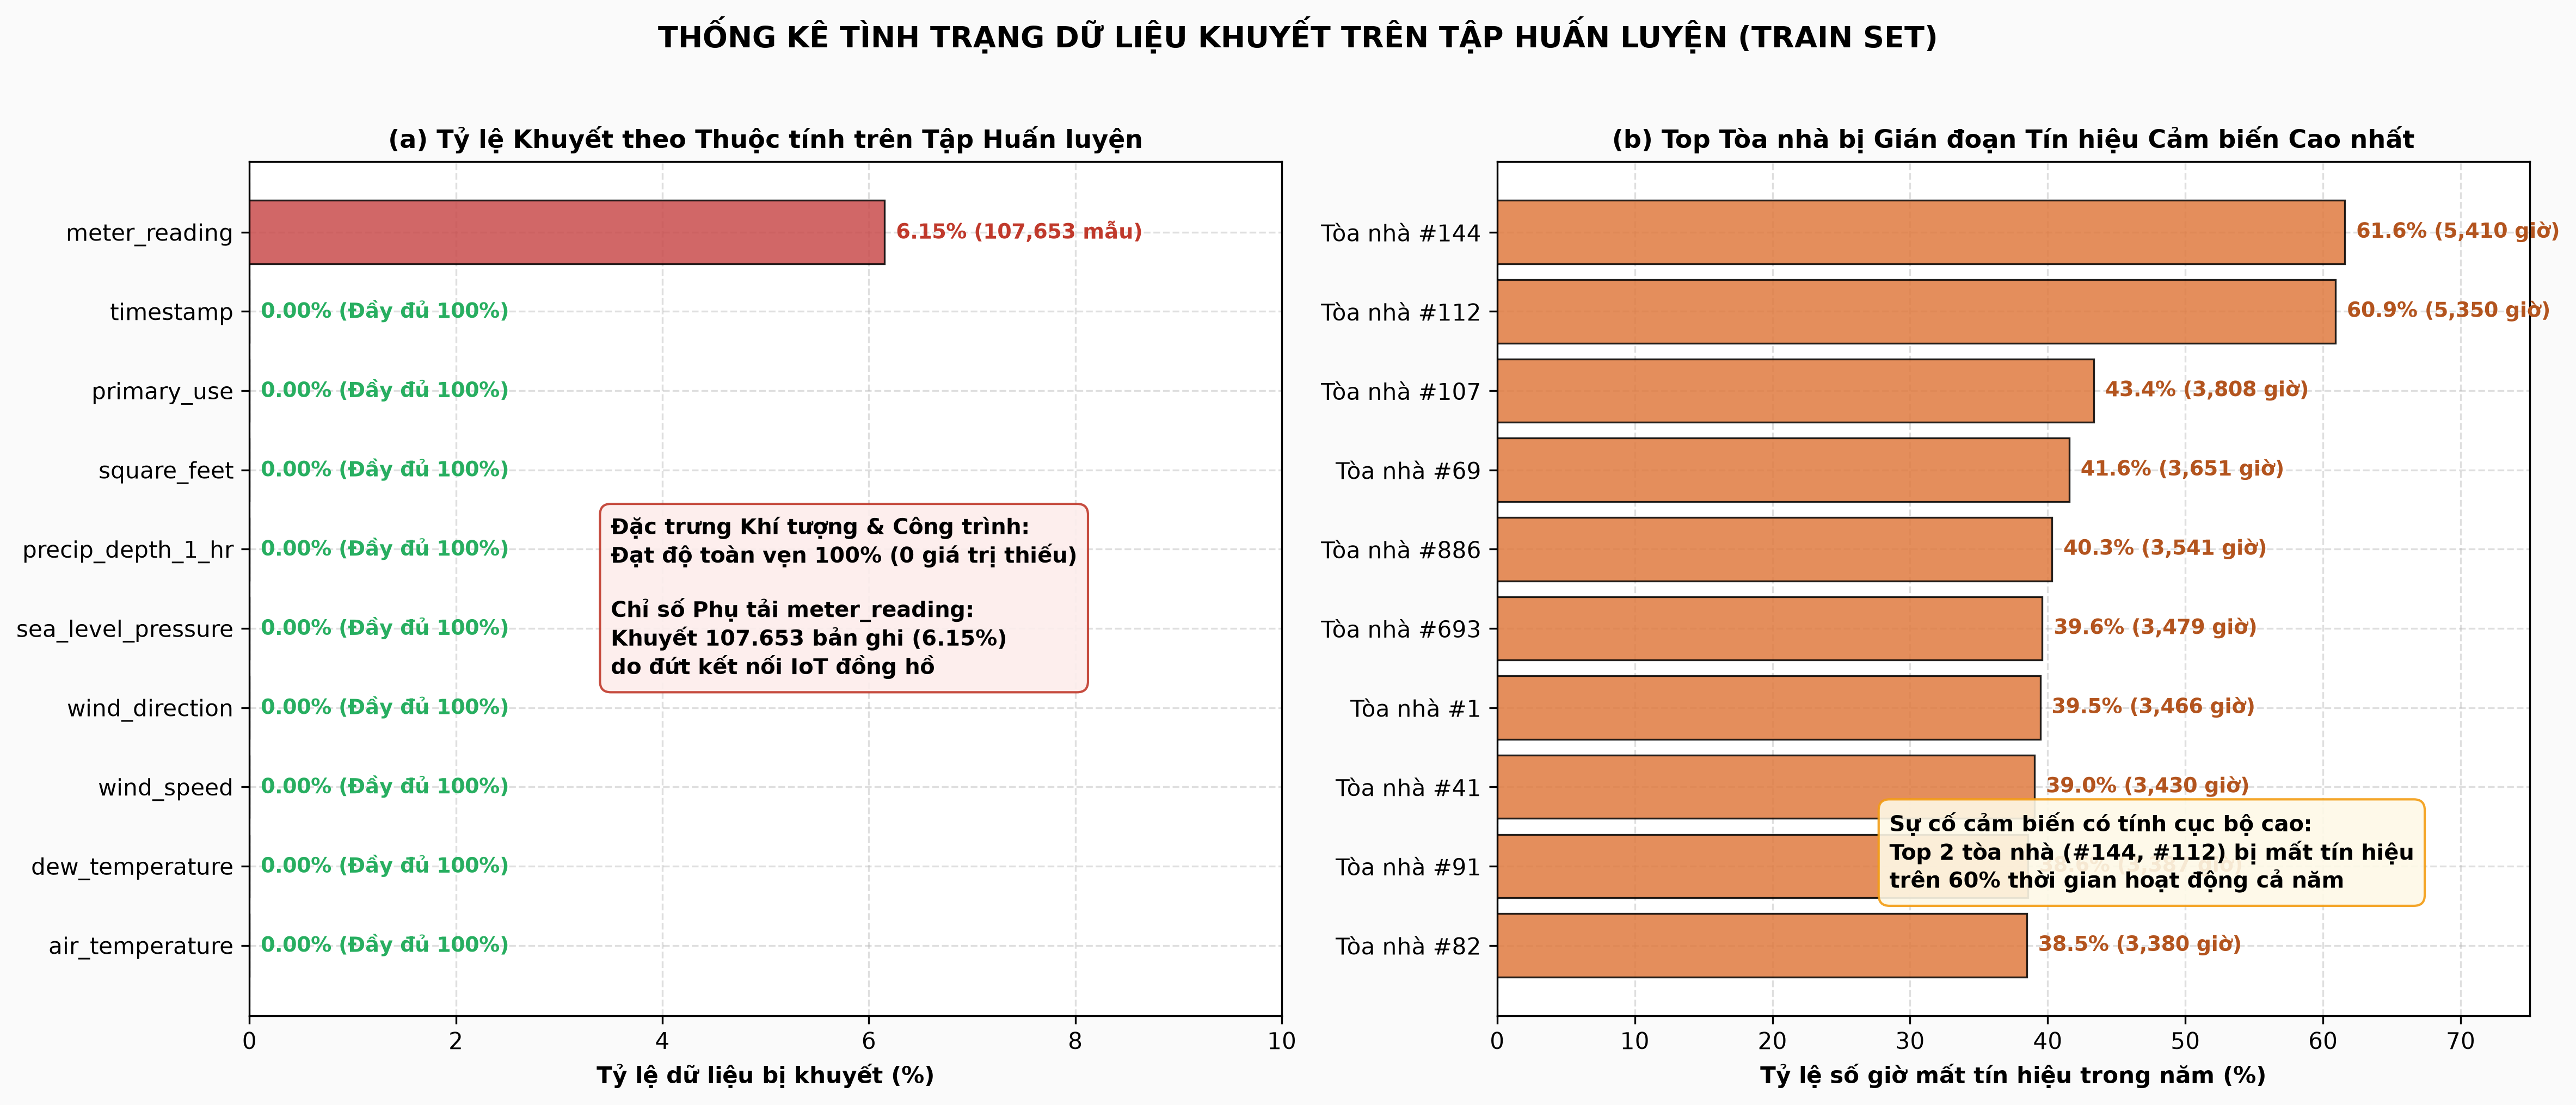
\includegraphics[width=0.98\textwidth]{IMAGE/eda_missing_sensor_noise.png}
    \caption{\textbf{Thống kê Tình trạng Dữ liệu Khuyết trên Tập Huấn luyện: Tỷ lệ khuyết theo thuộc tính (trái) và Top Tòa nhà bị gián đoạn cảm biến phụ tải cao nhất (phải)}}
    \label{fig:missing_sensor_noise}
\end{figure}

Từ Hình~\ref{fig:missing_sensor_noise}, nhóm nghiên cứu ghi nhận hai kết luận then chốt sau:
\begin{enumerate}
    \item \textbf{Tỷ lệ khuyết theo thuộc tính phụ tải (biểu đồ trái):} Thuộc tính phụ tải \texttt{meter\_reading} bị khuyết đúng $107.653$ bản ghi (chiếm tỷ lệ $6{,}15\%$ tổng số mẫu). Đáng chú ý, toàn bộ các thuộc tính thời tiết môi trường (\texttt{air\_temperature}, \texttt{dew\_temperature}, \texttt{wind\_speed}, \dots) cùng tem thời gian \texttt{timestamp} và quy mô công trình \texttt{square\_feet} đều đạt độ toàn vẹn $100\%$ ($0$ giá trị thiếu). Điều này khẳng định hệ thống trạm khí tượng hoạt động hoàn toàn ổn định, nguyên nhân thiếu dữ liệu thuần túy do kết nối truyền thông IoT từ đồng hồ thông minh về máy chủ đo lường bị ngắt quãng cục bộ.
    \item \textbf{Tính cục bộ của sự cố cảm biến (biểu đồ phải):} Dữ liệu thiếu không phân bố rải rác đồng đều giữa các công trình mà tập trung nghiêm trọng tại một số tòa nhà cá biệt. Điển hình như Tòa nhà \#144 bị mất tín hiệu $5.410$ giờ ($61{,}6\%$) và Tòa nhà \#112 bị mất $5.350$ giờ ($60{,}9\%$) dữ liệu trong năm (trên tổng số $8.784$ giờ của năm nhuận 2016). Việc mất tín hiệu kéo dài hàng ngàn giờ liên tiếp đặt ra yêu cầu quy trình tiền xử lý phải có giải pháp điền khuyết chuỗi thời gian phù hợp (nội suy tuyến tính kết hợp \textit{forward/backward fill} theo từng tòa nhà), tránh làm biến dạng quy luật phụ tải thực tế.
\end{enumerate}

\subsection{Quy trình Tiền xử lý Dữ liệu}

Nhằm chuẩn bị không gian đặc trưng tối ưu và triệt tiêu hoàn toàn rủi ro rò rỉ dữ liệu chuỗi thời gian, quy trình tiền xử lý được chuẩn hóa theo giao thức nghiêm ngặt và chia tách chu kỳ mùa vụ kết hợp khoảng đệm cách ly (Seasonal Chunking with 96h Purge Gap). Toàn bộ các thao tác nạp dữ liệu và khám phá sơ bộ đã được trình bày độc lập tại Mục~3.1.

Đặc biệt, trong nghiên cứu này, nhóm chủ động thiết kế quy trình nhằm tạo ra song song \textbf{ba bộ dữ liệu thực nghiệm tăng tiến phân cấp}:
\begin{enumerate}
    \item \textbf{Bộ dữ liệu cơ sở (Baseline Dataset - 39 đặc trưng / 40 cột):} Bao gồm đầy đủ các đặc trưng phụ tải, khí tượng, biến chu kỳ lượng giác và đặc tính công trình sau chuẩn hóa chuẩn mực.
    \item \textbf{Bộ dữ liệu mở rộng khu vực (Zone-enhanced Dataset - 42 đặc trưng / 43 cột):} Được tích hợp bổ sung 3 đặc trưng tương tác vùng khí hậu và quy mô công trình theo địa bàn (\texttt{zone\_interaction}, \texttt{site\_sqft\_mean}, \texttt{use\_sqft\_mean}).
    \item \textbf{Bộ dữ liệu ngữ cảnh vi mô nâng cao (Context-Aware Dataset - 46 đặc trưng / 47 cột):} Kế thừa trọn vẹn 42 đặc trưng của nhánh Zone và tích hợp thêm 4 đặc trưng vi mô chuẩn hóa phụ tải cục bộ của từng công trình (\texttt{z\_meter\_local}, \texttt{z\_meter\_workday}, \texttt{z\_meter\_robust}, \texttt{temp\_load\_inter}).
\end{enumerate}
Mục tiêu cốt lõi của việc thiết kế 3 bộ dữ liệu là phục vụ chuỗi đối chứng thực nghiệm tăng tiến: làm sáng tỏ năng lực phân tách khi bổ sung vùng Zone và bước đột phá hiệu năng khi tích hợp Context.

\subsubsection{Giao thức Phân chia Chuỗi Thời gian Chu kỳ Mùa vụ và 96 Giờ Cách ly (100\% Zero Data Leakage)}
Nhằm triệt tiêu tuyệt đối nguy cơ rò rỉ thông tin trong chuỗi thời gian (đặc biệt là tác động của các biến trễ khí tượng dài hạn \texttt{air\_temperature\_*\_lag73}), dữ liệu được phân chia theo giao thức Seasonal Chunking kết hợp khoảng cách ly Purge Gap 96 giờ:
\begin{itemize}
    \item \textbf{Tập Huấn luyện ($T_{\text{in}}$ - Train):} Chiếm các ngày từ $01$ đến $20$ hàng tháng ($1.147.089$ bản ghi, $\approx 65{,}6\%$). Toàn bộ các thống kê ($\mu, \sigma$, Median, IQR, các bảng tra cứu phụ tải) \textbf{chỉ được fit duy nhất trên tập này}.
    \item \textbf{Khoảng cách ly ($T_{\text{gap}}$ - Purge Gap 96h):} Chiếm các ngày từ $21$ đến $24$ hàng tháng ($229.412$ bản ghi, $\approx 13{,}1\%$). Khoảng đệm $96$ giờ này \textbf{bị loại bỏ hoàn toàn khỏi thực nghiệm}, tạo thành bức tường ngăn cách tuyệt đối giữa Train và Test.
    \item \textbf{Tập Kiểm định ($T_{\text{out}}$ - Test):} Chiếm từ ngày $25$ đến hết mỗi tháng ($372.993$ bản ghi, $\approx 21{,}3\%$). Tập này chỉ áp dụng phép chiếu (\textit{transform / map}) từ thống kê của Train, đóng vai trò là tập out-of-sample thực tế.
\end{itemize}

Chi tiết các bước biến đổi đặc trưng được triển khai tuần tự như sau:

\begin{enumerate}
    \item \textbf{Bước 1: Tách Nhãn mục tiêu và Định danh ra khỏi Ma trận Đặc trưng.}
    Vector nhãn $y_{\text{train}} = \texttt{anomaly}$ được tách riêng và đặt chỉ mục liên tục để phục vụ huấn luyện có giám sát, được loại bỏ khỏi ma trận đặc trưng $X_{\text{train}}$, bảo đảm mô hình không bị rò rỉ nhãn.

    \item \textbf{Bước 2: Chuẩn hóa Timestamp và Mã hóa Chu kỳ Thời gian ($\sin/\cos$).}
    Trường thời gian \texttt{timestamp} được ép kiểu sang định dạng \texttt{datetime64[ns]} chuẩn. Do thời gian có tính chu kỳ tuần hoàn khép kín, việc sử dụng giá trị số nguyên đơn thuần sẽ làm mất tính liên tục không gian. Do đó, các thành phần thời gian được mã hóa lượng giác trực tiếp:
    \begin{equation*}
        x_{\sin} = \sin\left(\frac{2\pi t}{T}\right), \quad x_{\cos} = \cos\left(\frac{2\pi t}{T}\right)
    \end{equation*}
    trong đó chu kỳ $T=24$ cho giờ trong ngày (\texttt{hour\_sin}, \texttt{hour\_cos}), $T=7$ cho ngày trong tuần (\texttt{weekday\_sin}, \texttt{weekday\_cos}), và $T=12$ cho tháng trong năm (\texttt{month\_sin}, \texttt{month\_cos}). Sau khi sinh các biến lượng giác, các cột thời gian gốc (\texttt{hour}, \texttt{weekday}, \texttt{month}) và các tọa độ thời gian cũ được loại bỏ hoàn toàn để tránh hiện tượng đa cộng tuyến.

    \item \textbf{Bước 3: Chuẩn hóa Lược đồ Đặc trưng, Phân loại Kiểu dữ liệu, Tạo Cờ Missing và Loại bỏ Đặc trưng không phù hợp.}
    \begin{itemize}
        \item \textbf{Tạo cờ missing:} Trước khi điền khuyết, nhóm khởi tạo biến cờ nhị phân:
        \begin{equation*}
            \texttt{meter\_reading\_was\_missing} = 
            \begin{cases}
                1, & \text{nếu } \texttt{meter\_reading} \text{ bị thiếu (NaN)} \\
                0, & \text{ngược lại}
            \end{cases}
        \end{equation*}
        Biến cờ này lưu giữ tín hiệu quan trọng về sự gián đoạn kết nối IoT của đồng hồ đo.
        \item \textbf{Chuẩn hóa lược đồ và phân nhóm kiểu dữ liệu:} Xác lập cấu trúc lược đồ chuẩn cho toàn bộ không gian đặc trưng; phân loại tường minh danh sách biến định lượng và biến định tính nhằm áp dụng quy trình xử lý chuyên biệt cho từng kiểu biến ở các bước kế tiếp.
        \item \textbf{Loại bỏ đặc trưng không phù hợp và Triệt tiêu Rò rỉ Nhãn Mục tiêu (Target Leakage):} Nhóm loại bỏ các biến hằng số không phương sai, các tổ hợp thời gian trùng lặp (\texttt{weekday\_hour}), và \textbf{đặc biệt quan trọng:} loại bỏ toàn bộ các biến mã hóa mục tiêu theo tòa nhà cá thể (\texttt{gte\_building\_id}, \texttt{gte\_meter\_}\allowbreak\texttt{building\_id}, \dots) cùng các đặc trưng gắn chặt với ID cụ thể của công trình (như \texttt{building\_weekday\_hour}, \texttt{building\_hour}, \dots). Quyết định kỹ thuật này dựa trên hai nguyên nhân cốt tử:
        \begin{enumerate}
            \item \textit{Nguy cơ Rò rỉ Dữ liệu Đích (Catastrophic Target Leakage):} Bản chất của Global Target Encoding (GTE) theo ID công trình là tính xác suất dị thường có điều kiện:
            \begin{equation*}
                \text{GTE}(\text{building\_id}=b) = \mathbb{E}[y \mid \text{building\_id} = b] = \frac{\sum_{i \in b} y_i}{N_b}
            \end{equation*}
            Nếu biến này được sinh ra trên toàn bộ tập dữ liệu trước khi phân chia chuỗi thời gian, thông tin nhãn mục tiêu $y$ từ tương lai ($T_{\text{out}}$) sẽ bị rò rỉ ngược hoàn toàn vào tập huấn luyện ($T_{\text{in}}$), tạo ra kết quả kiểm thử ảo tưởng và vi phạm nghiêm trọng nguyên tắc Zero Data Leakage.
            \item \textit{Nguy cơ Quá khớp Ghi nhớ ID (High-Cardinality Target Memorization):} Ngay cả khi được tính riêng trên $T_{\text{in}}$, do tập dữ liệu có tới $1.449$ tòa nhà cá biệt (lực lượng phân loại cực lớn), việc mã hóa nhãn mục tiêu trực tiếp cho từng ID sẽ biến các đặc trưng này thành biến đại diện gần như hoàn hảo cho nhãn $y$. Mô hình cây sẽ bị dẫn dắt vào việc "học vẹt" và ghi nhớ máy móc tòa nhà nào thường xuyên bị lỗi trong lịch sử thay vì học các quy luật phụ tải vật lý tổng quát (độ lệch Z-score, nhiệt độ, công năng). Điều này khiến mô hình mất hoàn toàn năng lực tổng quát hóa khi một công trình trước đây hoạt động bình thường bất ngờ phát sinh sự cố trong tương lai.
        \end{enumerate}
        Trái ngược với \texttt{building\_id}, biến công năng \texttt{primary\_use} chỉ có 16 nhóm ngành lớn mang tính quy luật vật lý chung (giáo dục, bệnh viện, văn phòng...), do đó chỉ có \texttt{gte\_primary\_use} và \texttt{gte\_meter\_primary\_use} (được học nghiêm ngặt $100\%$ trên $T_{\text{in}}$) là được giữ lại.
    \end{itemize}

    \item \textbf{Bước 4: Điền giá trị thiếu cho Dữ liệu Định lượng bằng Nội suy Chuỗi thời gian.}
    Khác với các phép gán trung vị hoặc trung bình toàn cục làm biến dạng dáng điệu phụ tải, nhóm áp dụng phương pháp nội suy tuyến tính theo thời gian (\texttt{interpolate(method=\allowbreak'time')}) được tính toán độc lập trong từng tòa nhà (\texttt{building\_id}). Ở các khoảng biên đầu và cuối chuỗi, kỹ thuật \textit{forward fill} và \textit{backward fill} được kết hợp để lấp đầy $100\%$ dữ liệu thiếu mà vẫn tôn trọng xu hướng động học thực tế.

    \item \textbf{Bước 5: Xử lý Giá trị Ngoại lai bằng Khoảng Tứ phân vị IQR.}
    Đối với các biến thời tiết môi trường (\texttt{air\_temperature}, \texttt{dew\_\allowbreak temperature}, \texttt{wind\_speed}, \dots), nhóm áp dụng quy tắc khoảng tứ phân vị IQR:
    \begin{equation*}
        \text{IQR} = Q_3 - Q_1, \quad [\text{Ngưỡng dưới}, \text{Ngưỡng trên}] = [Q_1 - 1{,}5\text{IQR}, \, Q_3 + 1{,}5\text{IQR}]
    \end{equation*}
    Các quan trắc thời tiết vượt ra ngoài khoảng này do lỗi thiết bị đo khí tượng được clip về giá trị trung vị cục bộ. 
    
    \textbf{Đặc biệt lưu ý:} Thuộc tính phụ tải \texttt{meter\_reading} và các đặc trưng Target Encoding (\texttt{gte\_}) được miễn trừ hoàn toàn khỏi bước này; việc ép phụ tải về trung vị sẽ trực tiếp triệt tiêu các mẫu dị thường mà mô hình cần nhận dạng.

    \item \textbf{Bước 6: Chuẩn hóa Z-score và Tích hợp Đặc trưng Khu vực.}
    \begin{itemize}
        \item \textbf{Chuẩn hóa Z-score:} Đưa các biến định lượng về phân phối có trung bình bằng 0 và độ lệch chuẩn bằng 1 bằng \texttt{StandardScaler}:
        \begin{equation*}
            Z = \frac{x - \mu}{\sigma}
        \end{equation*}
        Tham số $\mu, \sigma$ chỉ được fit trên tập huấn luyện và transform cho tập kiểm tra. Các biến cờ nhị phân ($0/1$), các biến chu kỳ $\sin/\cos \in [-1, 1]$, và các biến tỷ lệ \texttt{gte\_} $\in [0, 1]$ được giữ nguyên thang đo gốc.
        \item \textbf{Tích hợp Đặc trưng Khu vực:} Để tạo ra bộ dữ liệu Zone-enhanced phục vụ các bài toán phân hóa địa bàn, nhóm nghiên cứu xây dựng thêm 3 đặc trưng tương tác địa lý với quy cách mã hóa và ý nghĩa thực tế chi tiết như sau:
        \begin{enumerate}
            \item $\texttt{zone\_interaction}$: \textbf{Mã hóa tương tác phi tuyến giữa Vùng khí hậu và Mục đích sử dụng công trình}.
            \begin{itemize}
                \item \textit{Quy trình mã hóa:} Thuộc tính phân loại \texttt{primary\_use} trước hết được ánh xạ sang mã danh mục tạm thời $\texttt{primary\_use\_cat} \in \{0, 1, \dots, 11\}$ (ví dụ: \texttt{Education} = 0, \texttt{Entertainment} = 1, \dots). Sau đó, thực hiện phép ghép chuỗi ký tự giữa mã khu vực \texttt{site\_id} và mã công năng:
                \begin{equation*}
                    \text{Chuỗi tương tác} = \texttt{site\_id} \,\|\, \text{`\_'} \,\|\, \texttt{primary\_use\_cat}
                \end{equation*}
                Chuỗi này tiếp tục được chuyển hóa thành mã định danh số nguyên phân loại:
                \begin{equation*}
                    \texttt{zone\_interaction} = \text{CatCodes}(\text{Chuỗi tương tác}) \in \{0, 1, 2, \dots, 46\}
                \end{equation*}
                \item \textit{Ví dụ giá trị cụ thể:} 
                \begin{itemize}
                    \item Một tòa nhà trường học (\texttt{Education}, mã 0) tọa lạc tại Khu vực nhiệt đới \texttt{Site 0} sẽ có chuỗi ghép \texttt{"0\_0"}, được mã hóa thành giá trị nguyên $\mathbf{0}$. Trong khi đó, một trường học tương tự nhưng tọa lạc tại Khu vực ôn đới lạnh \texttt{Site 1} có chuỗi \texttt{"1\_0"}, được mã hóa thành giá trị $\mathbf{19}$; và tại \texttt{Site 2} có chuỗi \texttt{"2\_0"} nhận giá trị $\mathbf{24}$.
                    \item Một tòa nhà văn phòng (\texttt{Office}, mã 6) tại \texttt{Site 0} có chuỗi \texttt{"0\_6"} nhận giá trị $\mathbf{1}$, nhưng tại \texttt{Site 1} chuỗi \texttt{"1\_6"} nhận giá trị $\mathbf{22}$.
                \end{itemize}
                Toàn bộ dữ liệu ghi nhận chính xác 47 tổ hợp phân vùng thực tế (nhận giá trị từ 0 đến 46).
                \item \textit{Ý nghĩa đối với mô hình:} Biến tương tác này cho phép các thuật toán cây (LightGBM, XGBoost, CatBoost) thực hiện ngay lập tức một điểm cắt nhị phân (\textit{single-split decision}) để phân lập hành vi tiêu thụ điện đặc thù theo từng địa phương mà không cần phải thực hiện 2 đến 3 tầng phân nhánh liên tiếp.
            \end{itemize}

            \item $\texttt{site\_sqft\_mean}$: \textbf{Quy mô diện tích sàn trung bình của từng khu vực đô thị (\texttt{site\_id})}.
            \begin{itemize}
                \item \textit{Công thức tính:} Tính trung bình diện tích sàn của toàn bộ các công trình thuộc cùng một khu vực địa lý:
                \begin{equation*}
                    \texttt{site\_sqft\_mean}_i = \frac{1}{|S_{\texttt{site\_id}_i}|} \sum_{k \in S_{\texttt{site\_id}_i}} \texttt{square\_feet}_k
                \end{equation*}
                \item \textit{Ví dụ giá trị cụ thể:} Khu vực \texttt{Site 0} có diện tích bình quân $\mathbf{83.051{,}6\,\text{ft}^2}$ (đa số là khuôn viên trường đại học quy mô vừa); Khu vực \texttt{Site 4} tập trung các tổ hợp công nghệ lớn với diện tích bình quân lên tới $\mathbf{234.903{,}6\,\text{ft}^2}$; Khu vực siêu đô thị \texttt{Site 7} có diện tích sàn bình quân đạt đỉnh $\mathbf{484.376{,}0\,\text{ft}^2}$; trong khi Khu vực \texttt{Site 8} chủ yếu là các công trình nhỏ với diện tích trung bình chỉ $\mathbf{7.143{,}5\,\text{ft}^2}$.
                \item \textit{Ý nghĩa:} Cung cấp bối cảnh về mật độ và quy mô xây dựng đô thị tổng thể, giúp mô hình phân biệt giữa cụm đô thị dày đặc tải lớn và vùng phụ tải phân tán.
            \end{itemize}

            \item $\texttt{use\_sqft\_mean}$: \textbf{Quy mô diện tích sàn trung bình theo nhóm công năng (\texttt{primary\_use})}.
            \begin{itemize}
                \item \textit{Công thức tính:} Tính trung bình diện tích sàn của toàn bộ các công trình có cùng mục đích sử dụng:
                \begin{equation*}
                    \texttt{use\_sqft\_mean}_i = \frac{1}{|U_{\texttt{primary\_use}_i}|} \sum_{k \in U_{\texttt{primary\_use}_i}} \texttt{square\_feet}_k
                \end{equation*}
                \item \textit{Ví dụ giá trị cụ thể:} Nhóm công năng Dịch vụ phức hợp (\texttt{Services}) có diện tích trung bình cao nhất đạt $\mathbf{299.222{,}0\,\text{ft}^2}$; Nhà để xe (\texttt{Parking}) đạt $\mathbf{204.312{,}0\,\text{ft}^2}$; Trường học (\texttt{Education}) đạt $\mathbf{123.858{,}0\,\text{ft}^2}$; Văn phòng (\texttt{Office}) đạt $\mathbf{89.883{,}9\,\text{ft}^2}$; Sản xuất, công nghiệp (\texttt{Manufacturing} / \texttt{Industrial} )đạt $\mathbf{33.850{,}0\,\text{ft}^2}$; và nhóm công trình phụ trợ khác (\texttt{Other}) chỉ đạt $\mathbf{4.482{,}0\,\text{ft}^2}$.
                \item \textit{Ý nghĩa:} Đóng vai trò làm mốc đối chứng chuẩn mực theo loại hình. Khi kết hợp với diện tích sàn thực tế $\texttt{square\_feet}$, mô hình có thể tự động lượng hóa tỷ lệ lệch quy mô của một tòa nhà so với chuẩn mực ngành.
            \end{itemize}
        \end{enumerate}
        Sự hiện diện của 3 thuộc tính này chính là điểm phân tách cốt lõi giữa hai bộ dữ liệu thực nghiệm (Baseline: 39 đặc trưng vs Zone-enhanced: 42 đặc trưng). Bảng~\ref{tab:zone_sample_values} minh họa dữ liệu mẫu thực tế của 3 đặc trưng Zone trên các công trình đại diện trích xuất trực tiếp từ tập dữ liệu huấn luyện:

        \begin{table}[H]
        \centering
        \caption{\textbf{Mẫu dữ liệu thực nghiệm minh họa 3 đặc trưng Zone trên các công trình tiêu biểu}}
        \label{tab:zone_sample_values}
        \renewcommand{\arraystretch}{1.2}
        \resizebox{0.95\textwidth}{!}{
        \begin{tabular}{|c|c|l|r|c|c|c|}
        \hline
        \textbf{Building ID} & \textbf{Site ID} & \textbf{Công năng (\texttt{primary\_use})} & \textbf{Diện tích gốc (sqft)} & \texttt{zone\_interaction} & \texttt{site\_sqft\_mean} & \texttt{use\_sqft\_mean} \\ \hline
        1 & 0 & Education (Trường học) & 2.720 & 0 & -0,6202 & +0,2951 \\ \hline
        91 & 0 & Education (Trường học) & 68.094 & 0 & -0,6202 & +0,2951 \\ \hline
        32 & 0 & Office (Văn phòng) & 48.392 & 1 & -0,6202 & -0,1428 \\ \hline
        136 & 1 & Lodging/residential & 56.467 & 21 & -0,0238 & -0,5030 \\ \hline
        240 & 2 & Lodging/residential & 111.304 & 26 & +0,1275 & -0,5030 \\ \hline
        69 & 0 & Parking (Nhà để xe) & 387.638 & 2 & -0,6202 & -0,5826 \\ \hline
        \end{tabular}
        }
        \end{table}
    \end{itemize}

    \item \textbf{Bước 7: Tích hợp Đặc trưng Ngữ cảnh (Context-Aware Feature Engineering).}
    Mặc dù 3 đặc trưng Zone cung cấp thông tin vĩ mô cấp khu vực, mức tiêu thụ điện thực tế lại phụ thuộc trực tiếp vào nhịp sinh hoạt và chế độ vận hành riêng của từng công trình cá biệt. Do đó, nhóm nghiên cứu thiết kế thêm 4 đặc trưng vi mô chuẩn hóa Z-score cục bộ, được học 100\% trên tập huấn luyện $T_{\text{in}}$ (100\% Zero Data Leakage) và ánh xạ sang tập kiểm định $T_{\text{out}}$:
    \begin{enumerate}
        \item $\texttt{z\_meter\_local}$: Phụ tải chuẩn hóa theo cặp $(\texttt{building\_id}, \texttt{hour})$. Cho biết mức độ chênh lệch của phụ tải hiện tại so với hành vi bình thường của tòa nhà vào đúng khung giờ đó:
        \begin{equation*}
            \texttt{z\_meter\_local}_i = \frac{\texttt{meter\_reading}_i - \mu_{(b, h)}}{\sigma_{(b, h)}}
        \end{equation*}
        \item $\texttt{z\_meter\_workday}$: Phụ tải chuẩn hóa theo bộ ba $(\texttt{building\_id}, \texttt{is\_offday}, \texttt{hour})$. Tách biệt rõ nét giữa ngày làm việc thông thường và ngày nghỉ/cuối tuần (nơi phụ tải nền thường giảm mạnh):
        \begin{equation*}
            \texttt{z\_meter\_workday}_i = \frac{\texttt{meter\_reading}_i - \mu_{(b, \text{off}, h)}}{\sigma_{(b, \text{off}, h)}}
        \end{equation*}
        \item $\texttt{z\_meter\_robust}$: Chuẩn hóa kháng nhiễu (\textit{Robust Z-score}) dựa trên Trung vị và Khoảng tứ phân vị của từng công trình:
        \begin{equation*}
            \texttt{z\_meter\_robust}_i = \frac{\texttt{meter\_reading}_i - \text{Median}_b}{\text{IQR}_b}
        \end{equation*}
        Nhờ dùng Trung vị và IQR thay vì Mean và Std, đặc trưng này không bị lệch lạc bởi các giá trị dị thường cực đoan.
        \item $\texttt{temp\_load\_inter}$: Đặc trưng tương tác giữa phụ tải công việc và nhiệt độ không khí môi trường:
        \begin{equation*}
            \texttt{temp\_load\_inter}_i = \texttt{z\_meter\_workday}_i \times \texttt{air\_temperature}_i
        \end{equation*}
    \end{enumerate}
    Sự bổ sung của 4 đặc trưng này hoàn thiện biến thể thứ ba: \textbf{Context-Aware Dataset} gồm đúng \textbf{46 đặc trưng} (\textbf{47 cột} tính cả nhãn mục tiêu \texttt{anomaly}). Bảng~\ref{tab:context_sample_values} trình bày mẫu dữ liệu thực nghiệm trích xuất trực tiếp từ tập dữ liệu huấn luyện $T_{\text{in}}$, đối chiếu định lượng giữa các trạng thái vận hành bình thường ($y=0$) và các dạng thức dị thường điển hình ($y=1$) bao gồm quá tải phụ tải điện, sụt giảm đứt gãy phụ tải nền, và bất thường lệch nhịp công tác:

    \begin{table}[H]
    \centering
    \caption{\textbf{Mẫu dữ liệu thực nghiệm minh họa 4 đặc trưng Context-Aware trên các công trình tiêu biểu}}
    \label{tab:context_sample_values}
    \renewcommand{\arraystretch}{1.2}
    \resizebox{\textwidth}{!}{
    \begin{tabular}{|c|c|l|c|c|c|c|c|c|c|}
    \hline
    \textbf{Building} & \textbf{Site} & \textbf{Công năng chính} & \textbf{Trạng thái vận hành} & \texttt{meter} & \texttt{Temp} & \texttt{z\_local} & \texttt{z\_work} & \texttt{z\_robust} & \texttt{temp\_inter} \\ \hline
    1 & 0 & Education (Trường học) & Bình thường ($y=0$) & -0,234 & -0,15 & +1,1444 & +1,1535 & +0,9537 & -0,1780 \\ \hline
    1 & 0 & Education (Trường học) & Dị thường ($y=1$) (Sụt tải) & -0,418 & +0,90 & -1,6408 & -1,6218 & -0,5629 & -1,4522 \\ \hline
    32 & 0 & Office (Văn phòng) & Bình thường ($y=0$) & -0,234 & -0,15 & +0,7961 & +0,6676 & 0,0000 & -0,1030 \\ \hline
    32 & 0 & Office (Văn phòng) & Dị thường ($y=1$) (Trái nhịp) & -0,208 & +0,73 & +0,1678 & +0,8362 & +0,2684 & +0,6079 \\ \hline
    136 & 1 & Lodging/residential & Bình thường ($y=0$) & -0,381 & -1,02 & -0,8744 & -0,8920 & -0,3164 & +0,9062 \\ \hline
    136 & 1 & Lodging/residential & Dị thường ($y=1$) (Đứt gãy tải) & -0,370 & -1,27 & -0,6715 & -0,6887 & -0,2097 & +0,8770 \\ \hline
    1128 & 13 & Office (Văn phòng) & Dị thường ($y=1$) (Đột biến đỉnh) & +0,480 & -3,02 & +10,0000 & +9,4721 & +7,4612 & -28,5724 \\ \hline
    144 & 1 & Office (Văn phòng) & Dị thường ($y=1$) (Triệt tiêu tải) & -0,450 & -1,24 & -5,0000 & -5,0000 & -2,1934 & +6,2158 \\ \hline
    69 & 0 & Parking (Nhà để xe) & Bình thường ($y=0$) & -0,234 & -0,15 & +1,1788 & +1,2004 & +0,6218 & -0,1853 \\ \hline
    69 & 0 & Parking (Nhà để xe) & Dị thường ($y=1$) (Bất thường tải) & -0,436 & +0,90 & -0,7673 & -0,7814 & -0,6900 & -0,6996 \\ \hline
    \end{tabular}
    }
    \end{table}

    \noindent \textbf{Phân tích định lượng từ mẫu dữ liệu thực nghiệm:}
    \begin{itemize}
        \item \textit{Độ nhạy phân lập trước các sự cố cực đoan:} Tại tòa nhà văn phòng \texttt{Building 1128}, sự cố tăng vọt phụ tải bất thường vào khung giờ nhiệt độ lạnh giá ($T=-3{,}02$) được bộ đôi \texttt{z\_meter\_local} và \texttt{z\_meter\_workday} phát hiện ngay tức thì khi chạm ngưỡng trần bão hòa $+10{,}0000$ và $+9{,}4721$, kết hợp với đặc trưng tương tác âm tính cực lớn $\texttt{temp\_load\_inter} = -28{,}5724$. Ngược lại, tại \texttt{Building 144}, hiện tượng mất phụ tải đột ngột kéo \texttt{z\_meter\_local} chạm ngưỡng sàn $-5{,}0000$.
        \item \textit{Bắt trúng dị thường ngữ cảnh vi mô (Contextual Anomalies):} Tại \texttt{Building 32}, phụ tải điện $\texttt{meter\_reading} = -0{,}208$ nếu chỉ nhìn dưới góc độ ngưỡng toàn cục sẽ bị nhầm lẫn là tiêu thụ bình thường (nhãn $y=0$ thông thường nhận $-0{,}234$). Tuy nhiên, tại thời điểm ngày nghỉ khi toàn bộ văn phòng đóng cửa, việc tiêu thụ mức này đẩy \texttt{z\_meter\_workday} lên $+0{,}8362$ và $\texttt{temp\_load\_inter} = +0{,}6079$, tạo tín hiệu rõ nét giúp mô hình phân định chính xác đây là điểm bất thường vận hành ngoài giờ.
    \end{itemize}
\end{enumerate}

\subsection{Khám phá Dữ liệu sau Tiền xử lý}

Sau khi hoàn tất toàn bộ chuỗi biến đổi tiền xử lý, nhóm nghiên cứu tiến hành kiểm toán dữ liệu và khám phá đối chiếu nhằm đánh giá toàn diện sự thay đổi của tập dữ liệu trước khi bước vào giai đoạn huấn luyện mô hình.

\subsubsection{Kiểm tra Tính Toàn vẹn và Phân bổ Đặc trưng}
Quá trình kiểm tra ràng buộc nghiêm ngặt trên bộ dữ liệu thực nghiệm sau tiền xử lý mang lại các kết quả kiểm toán sau:
\begin{enumerate}
    \item \textbf{Bảo toàn dữ liệu theo chu kỳ và triệt tiêu rò rỉ:} Dữ liệu phân chia theo tỷ lệ $T_{\text{in}}$ ($1.147.089$ dòng, $65{,}6\%$), Purge Gap ($229.412$ dòng, $13{,}1\%$), và $T_{\text{out}}$ ($372.993$ dòng, $21{,}3\%$).
    \item \textbf{Triệt tiêu hoàn toàn giá trị thiếu:} Toàn bộ các thuộc tính đạt tỷ lệ hoàn chỉnh $100\%$ ($0$ giá trị \texttt{NaN}) nhờ chiến lược nội suy chuỗi thời gian kết hợp cờ nhị phân ghi nhận mất tín hiệu.
    \item \textbf{Xác lập không gian đặc trưng chuẩn tắc cho ba nhánh dữ liệu tăng tiến:}
    \begin{itemize}
        \item \textit{Nhánh Cơ sở (Baseline Dataset):} Gồm đúng \textbf{39 đặc trưng cốt lõi} (\textbf{40 cột} tính cả nhãn mục tiêu \texttt{anomaly}).
        \item \textit{Nhánh Mở rộng Khu vực (Zone-enhanced Dataset):} Gồm đúng \textbf{42 đặc trưng} (\textbf{43 cột} tính cả nhãn \texttt{anomaly}), bổ sung $3$ đặc trưng tương tác phân vùng (\texttt{zone\_interaction}, \texttt{site\_sqft\_mean}, \texttt{use\_sqft\_mean}).
        \item \textit{Nhánh Ngữ cảnh Cục bộ SOTA (Context-Aware Dataset):} Gồm đúng \textbf{46 đặc trưng} (\textbf{47 cột} tính cả nhãn \texttt{anomaly}), kế thừa toàn bộ nhánh Zone và bổ sung $4$ đặc trưng Z-score vi mô (\texttt{z\_meter\_local}, \texttt{z\_meter\_workday}, \texttt{z\_meter\_robust}, \texttt{temp\_load\_inter}).
    \end{itemize}
\end{enumerate}

Bảng~\ref{tab:final_feature_summary} tổng hợp chi tiết cấu trúc các nhóm đặc trưng còn giữ lại trong không gian biểu diễn cuối cùng của hai bộ dữ liệu thực nghiệm.

\begin{table}[H]
\centering
\small
\setlength{\extrarowheight}{4pt}
\begin{tabularx}{\textwidth}{|>{\raggedright\arraybackslash}m{3.6cm}|>{\centering\arraybackslash}m{2.0cm}|>{\raggedright\arraybackslash}X|}
\hline
\textbf{Nhóm Đặc trưng} & \textbf{Số lượng} & \textbf{Các thuộc tính chi tiết và Ý nghĩa nghiệp vụ} \\
\hline
Đặc trưng Phụ tải gốc & 1 & \texttt{meter\_reading} (sau khi nội suy chuỗi thời gian và chuẩn hóa Z-score). \\
\hline
Cảm biến Khí tượng gốc & 7 & \texttt{air\_temperature}, \texttt{cloud\_coverage}, \texttt{dew\_temperature}, \texttt{precip\_depth\_1\_hr}, \texttt{sea\_level\_pressure}, \texttt{wind\_direction}, \texttt{wind\_speed} (sau lọc ngoại lai IQR và Z-score). \\
\hline
Chuỗi trễ Khí tượng & 8 & \texttt{air\_temperature\_mean\_lag7}, \texttt{max\_lag7}, \texttt{min\_lag7}, \texttt{std\_lag7} (trễ 7h trong ngày) kết hợp \texttt{mean\_lag73}, \texttt{max\_lag73}, \texttt{min\_lag73}, \texttt{std\_lag73} (trễ 73h theo đợt nhiệt). \\
\hline
Đặc tính Công trình \& ID & 5 & \texttt{square\_feet}, \texttt{year\_built}, \texttt{floor\_count} (quy mô, niên hạn) kết hợp \texttt{building\_id}, \texttt{site\_id} (định danh công trình và vùng địa lý). \\
\hline
Chu kỳ Lượng giác \& Lễ & 7 & \texttt{hour\_sin}, \texttt{hour\_cos}, \texttt{weekday\_sin}, \texttt{weekday\_cos}, \texttt{month\_sin}, \texttt{month\_cos} (chu kỳ 24h, 7 ngày, 12 tháng) và cờ ngày nghỉ \texttt{is\_holiday}. \\
\hline
Cờ Gián đoạn Cảm biến & 1 & \texttt{meter\_reading\_was\_missing} (lưu dấu vết sự cố truyền thông IoT trước khi điền khuyết). \\
\hline
Mã hóa Mục tiêu (GTE) & 10 & \texttt{gte\_hour}, \texttt{gte\_weekday}, \texttt{gte\_month}, \texttt{gte\_primary\_use}, \texttt{gte\_site\_id}, \texttt{gte\_meter\_hour}, \texttt{gte\_meter\_weekday}, \texttt{gte\_meter\_month}, \texttt{gte\_meter\_primary\_use}, \texttt{gte\_meter\_site\_id}. \\
\hline
\textbf{Tổng số đặc trưng Baseline} & \textbf{39} & \textbf{Ma trận đặc trưng Baseline hoàn chỉnh (40 cột tính cả nhãn \texttt{anomaly})}. \\
\hline
Tương tác Khu vực & 3 & \texttt{zone\_interaction}, \texttt{site\_sqft\_mean}, \texttt{use\_sqft\_mean} (phân hóa địa phương; chỉ có trên bộ Zone-enhanced). \\
\hline
\textbf{Tổng số đặc trưng Zone} & \textbf{42} & \textbf{Ma trận đặc trưng Zone-enhanced hoàn chỉnh (43 cột tính cả nhãn \texttt{anomaly})}. \\
\hline
Ngữ cảnh & 4 & \texttt{z\_meter\_local}, \texttt{z\_meter\_workday}, \texttt{z\_meter\_robust}, \texttt{temp\_load\_inter} (chuẩn hóa phụ tải cục bộ theo từng công trình; chỉ có trên bộ Context-Aware). \\
\hline
\textbf{Tổng số đặc trưng Context} & \textbf{46} & \textbf{Ma trận đặc trưng Context-Aware hoàn chỉnh (47 cột tính cả nhãn \texttt{anomaly})}. \\
\hline
\end{tabularx}
\caption{\textbf{Tổng hợp phân loại các nhóm đặc trưng trong ma trận dữ liệu qua 3 tầng (Baseline, Zone, Context)}}
\label{tab:final_feature_summary}
\end{table}

\begin{table}[H]
\centering
\caption{\textbf{Bảng kiểm toán biến đổi số dòng và thuộc tính qua 8 giai đoạn tiền xử lý (Zero Data Leakage)}}
\label{tab:preprocessing_audit_steps}
\renewcommand{\arraystretch}{1.2}
\resizebox{\textwidth}{!}{
\begin{tabular}{|l|r|r|r|r|r|r|c|}
\hline
\textbf{Giai đoạn Tiền xử lý} & \textbf{$T_{\text{in}}$ Trước} & \textbf{$T_{\text{in}}$ Sau} & \textbf{Purge Gap} & \textbf{$T_{\text{out}}$ Trước} & \textbf{$T_{\text{out}}$ Sau} & \textbf{Số cột} & \textbf{Ghi chú Rò rỉ} \\ \hline
1. Nạp CSV Thô & 1.749.494 & 1.749.494 & 0 & --- & --- & 57 & Dữ liệu thô nguyên bản \\ \hline
2. Seasonal Chunking \& 96h Purge Gap & 1.749.494 & 1.147.089 & 229.412 & --- & 372.993 & 57 & Loại bỏ 96h buffer \\ \hline
3. Khử 23 cột rò rỉ ID \& Mã hóa $\sin/\cos$ & 1.147.089 & 1.147.089 & 0 & 372.993 & 372.993 & 34 & Khử tuyệt đối ID leak \\ \hline
4. Cờ Missing \& Nội suy khuyết thiếu & 1.147.089 & 1.147.089 & 0 & 372.993 & 372.993 & 35 & 100\% sạch ($0{,}00\%$ NaN) \\ \hline
5. Lọc ngoại lai khí tượng (IQR) & 1.147.089 & 1.147.089 & 0 & 372.993 & 372.993 & 35 & Kẹp biên IQR/Median \\ \hline
6. Chuẩn hóa Z-score \& Nhánh Zone & 1.147.089 & 1.147.089 & 0 & 372.993 & 372.993 & 40 / 43 & Fit $T_{\text{in}}$, transform $T_{\text{out}}$ \\ \hline
7. Tích hợp Ngữ cảnh Context Vi mô & 1.147.089 & 1.147.089 & 0 & 372.993 & 372.993 & 47 & Fit lookup $T_{\text{in}}$, map $T_{\text{out}}$ \\ \hline
8. Xuất 6 bộ Parquet Chuẩn hóa & 1.147.089 & 1.147.089 & 0 & 372.993 & 372.993 & 40/43/47 & 3 cặp Train/Test độc lập \\ \hline
\end{tabular}
}
\end{table}

\subsubsection{Lược đồ Lịch sử Tiến trình Tiền xử lý}
Nhằm trực quan hóa tính liên tục và tính toàn vẹn của quá trình biến đổi dữ liệu qua từng giai đoạn, nhóm nghiên cứu xây dựng hàm \texttt{plot\_preprocessing\_history()} trong mô-đun kiểm toán dữ liệu để trích xuất lược đồ lịch sử tiền xử lý toàn diện tại Hình~\ref{fig:preprocessing_history}.

\begin{figure}[H]
    \centering
    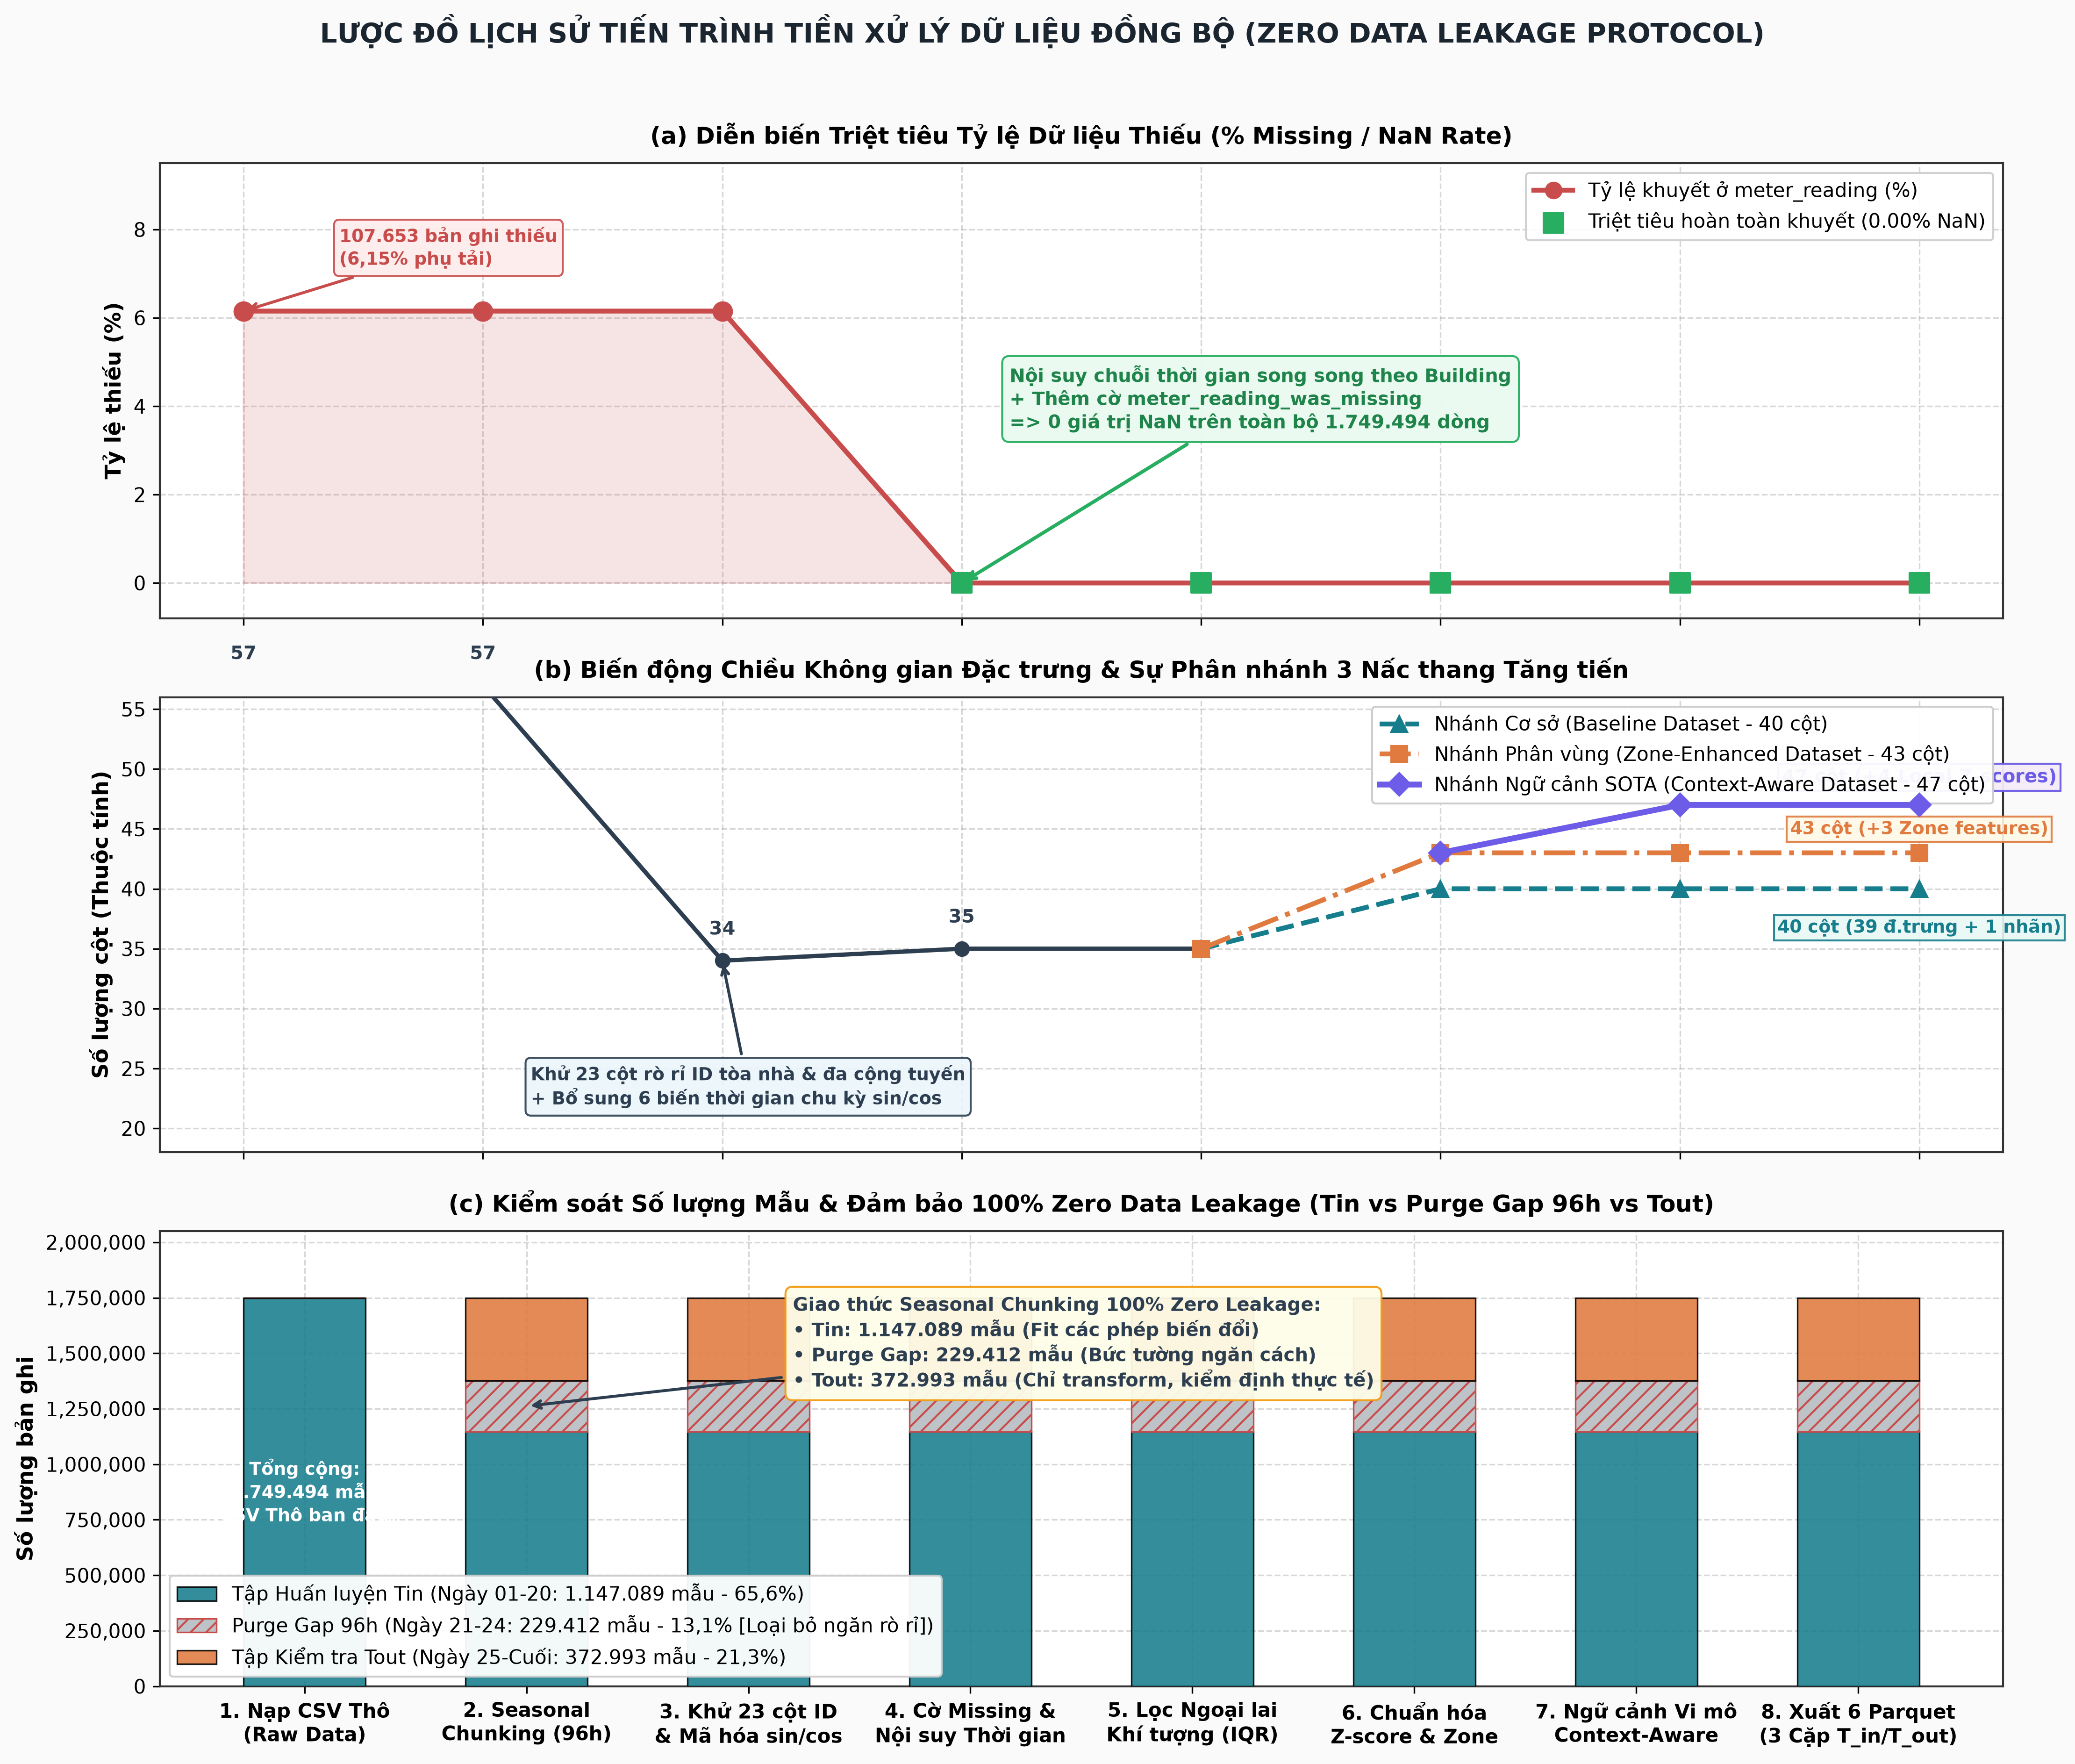
\includegraphics[width=0.98\textwidth]{IMAGE/preprocessing_history_diagram.png}
    \caption{\textbf{Lược đồ Lịch sử Tiền xử lý: Diễn biến triệt tiêu dữ liệu thiếu, biến động chiều không gian đặc trưng và kiểm soát mẫu Zero Data Leakage qua từng giai đoạn}}
    \label{fig:preprocessing_history}
\end{figure}

Lược đồ lịch sử tại Hình~\ref{fig:preprocessing_history} thể hiện rõ nét 3 khía cạnh kiểm toán khoa học:
\begin{itemize}
    \item \textbf{Về dữ liệu thiếu (Hình~\ref{fig:preprocessing_history}a):} Tỷ lệ khuyết $6{,}15\%$ ở biến phụ tải ($107.653$ bản ghi thiếu) được giải quyết triệt để sau bước nội suy chuỗi thời gian song song theo từng công trình (Bước 4), kết hợp bổ sung cờ nhị phân \texttt{meter\_reading\_was\_missing}, đưa toàn bộ hệ thống về trạng thái hoàn chỉnh tuyệt đối $0{,}00\%$ dữ liệu thiếu trước khi bước vào các phép toán chuẩn hóa.
    \item \textbf{Về không gian đặc trưng và sự phân nhánh (Hình~\ref{fig:preprocessing_history}b):} Số chiều đặc trưng xuất phát từ 57 cột ban đầu, mở rộng lên 63 cột sau khi mã hóa $\sin/\cos$ chu kỳ thời gian; sau đó được tinh giản mạnh về 34 cột nhờ kiên quyết loại bỏ 23 biến rò rỉ ID tòa nhà và các biến hằng số; bổ sung cờ missing đạt 35 cột; và cuối cùng phân nhánh thành công thành ba không gian tăng tiến: \textbf{Baseline (40 cột)}, \textbf{Zone-Enhanced (43 cột)} và \textbf{Context-Aware SOTA (47 cột)}.
    \item \textbf{Về kiểm soát mẫu và ngăn ngừa rò rỉ thời gian (Hình~\ref{fig:preprocessing_history}c):} Toàn bộ $1.749.494$ bản ghi được phân bổ nghiêm ngặt theo giao thức Seasonal Chunking: tập huấn luyện $T_{\text{in}}$ ($1.147.089$ dòng, $65{,}6\%$), vùng đệm cách ly Purge Gap 96 giờ ($229.412$ dòng, $13{,}1\%$, bị loại bỏ hoàn toàn để triệt tiêu ảnh hưởng tự tương quan của biến trễ \texttt{lag73}), và tập kiểm định out-of-sample $T_{\text{out}}$ ($372.993$ dòng, $21{,}3\%$).
\end{itemize}

\subsubsection{Khám phá và Động lực Khoa học của Tương tác Khu vực (Zone EDA)}
Để làm rõ vì sao nhóm nghiên cứu quyết định phát triển song song ba bộ dữ liệu tăng tiến (Baseline, Zone-enhanced, Context-Aware), hàm phân tích \texttt{plot\_eda\_zone\_comparison()} được triển khai để trực quan hóa sự phân hóa thực tế về phụ tải và nhiệt độ giữa các khu vực địa lý tiêu biểu (\texttt{site\_id} 0, 2, 4, 9, Hình~\ref{fig:zone_comparison}).

\begin{figure}[H]
    \centering
    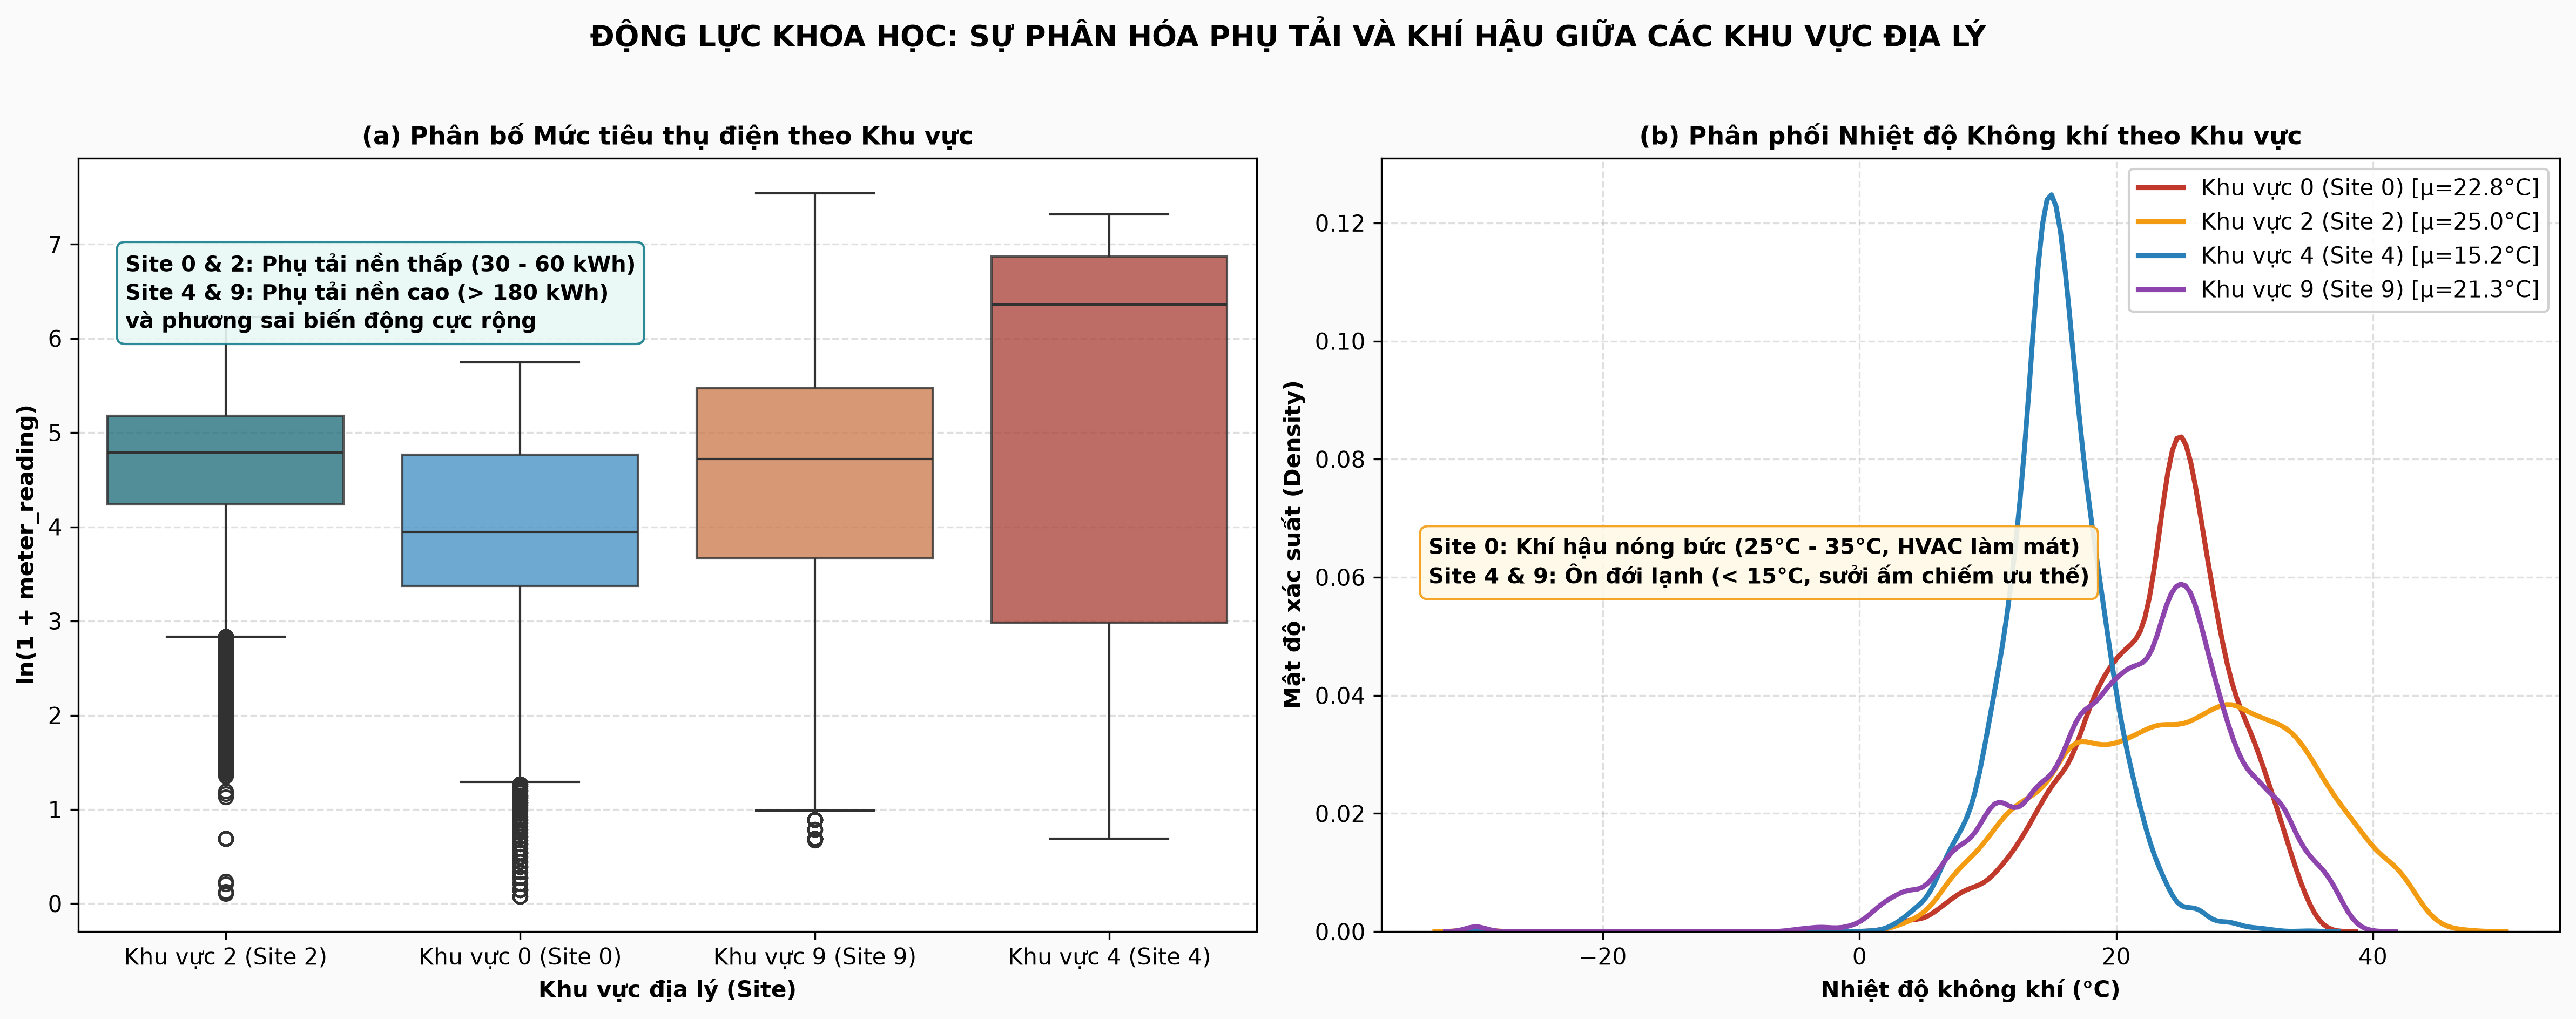
\includegraphics[width=0.98\textwidth]{IMAGE/eda_zone_comparison.png}
    \caption{\textbf{Phân bố Mức tiêu thụ điện (trái) và Phân phối Nhiệt độ (phải) giữa các Khu vực (Site 0, 2, 4, 9)}}
    \label{fig:zone_comparison}
\end{figure}

Phân tích Hình~\ref{fig:zone_comparison} cho thấy hai quy luật môi trường mang tính quyết định:
\begin{itemize}
    \item \textbf{Sự phân cực về mức tiêu thụ (biểu đồ trái):} Khu vực Site 0 và Site 2 có trung vị phụ tải thấp ($30 - 60\,\text{kWh}$) với biên độ dao động hẹp, trong khi Site 4 và Site 9 tiêu thụ liên tục ở mức rất cao ($>180\,\text{kWh}$) và xuất hiện nhiều đuôi phân phối kéo dài.
    \item \textbf{Sự sai khác về đới khí hậu (biểu đồ phải):} Nhiệt độ không khí tại Site 0 tập trung chủ yếu trong vùng nóng ($25^\circ\text{C} - 35^\circ\text{C}$), đòi hỏi hệ thống điều hòa HVAC chạy liên tục. Ngược lại, Site 4 và Site 9 nằm trong đới khí hậu ôn đới lạnh với nhiệt độ chủ yếu dưới $15^\circ\text{C}$, nơi nhu cầu sưởi ấm chiếm ưu thế.
\end{itemize}

Nếu chỉ sử dụng bộ dữ liệu cơ sở (Baseline) mà không tích hợp đặc trưng Zone và đặc trưng Context-Aware, mô hình học máy sẽ bị ép phải khớp một hàm mục tiêu trung bình hóa trên toàn bộ 16 khu vực, dẫn đến việc ngộ nhận một mức phụ tải $100\,\text{kWh}$ tại Site 0 là dị thường (trong khi ở Site 4 đó lại là mức tải nền bình thường). 

Chính vì vậy, việc xây dựng **ba bộ dữ liệu tăng tiến (Baseline, Zone-enhanced và Context-Aware)** cho phép nhóm nghiên cứu tiến hành đánh giá thực nghiệm đa chiều ở Chương 4, qua đó xác thực một cách định lượng sự bứt phá hiệu năng khi tích hợp bối cảnh khu vực và ngữ cảnh vào các thuật toán học máy.